\documentclass[a4paper,12pt]{article}
\usepackage{geometry}
\geometry{left=3cm,right=3cm,top=3cm,bottom=3cm,footskip=2cm}
\usepackage{setspace}
\linespread{1.3}

\usepackage{lmodern}
\usepackage{amssymb,amsmath}
%\usepackage{ifxetex,ifluatex}
%\usepackage{fixltx2e} % provides \textsubscript
\usepackage[T1]{fontenc}
\usepackage[utf8]{inputenc}
\usepackage{eurosym}
%\usepackage{natbib}
%\bibliographystyle{plainnat}
%\usepackage{biblatex}
%\bibliography{}
\usepackage{listings}
%Allow degree escape in listings
\usepackage{gensymb}
\usepackage{color}
\definecolor{lightgray}{gray}{0.60}
\definecolor{lightgraycode}{gray}{0.80}
\definecolor{keywords}{RGB}{255,0,90}
\definecolor{comments}{RGB}{76,76,76}
\definecolor{string}{RGB}{0,0,250}
\definecolor{identifier}{RGB}{250,80,0}
\definecolor{tag}{rgb}{0,0.46,0}

\lstset{
  basicstyle=\ttfamily \lst@ifdisplaystyle\scriptsize\fi,
  framexleftmargin = 5mm,
  frame            = shadowbox,
  rulesepcolor     = \color{lightgraycode},
  numbers          = left,
  numberstyle      = \tiny,
  numbersep        = 10pt,
  columns          = fullflexible,
  breaklines       = true,
  showstringspaces = false,
  commentstyle     = \color{comments}\upshape
}

\lstdefinelanguage{XML}
{
  morestring=[b]",
  morestring=[s]{>}{<},
  morecomment=[s]{<?}{?>},
  morecomment=[s]{--}{--},
  moredelim=[s][\color{keywords}]{\ }{=},
  stringstyle=\color{black},
  identifierstyle=\color{tag},
}

\usepackage{longtable,booktabs}
\usepackage{graphicx}
\usepackage{pdfpages}
\makeatletter
\def\maxwidth{\ifdim\Gin@nat@width>\linewidth\linewidth\else\Gin@nat@width\fi}
\def\maxheight{\ifdim\Gin@nat@height>\textheight\textheight\else\Gin@nat@height\fi}
\makeatother
% Scale images if necessary, so that they will not overflow the page
% margins by default, and it is still possible to overwrite the defaults
% using explicit options in \includegraphics[width, height, ...]{}
\setkeys{Gin}{width=\maxwidth,height=\maxheight,keepaspectratio}
\usepackage[unicode=true]{hyperref}
\hypersetup{breaklinks=true,
            bookmarks=true,
            pdfauthor=Esteban Munoz,
            pdftitle=Guidelines Energy-ADE,
            colorlinks=true,
            citecolor=blue,
            urlcolor=blue,
            linkcolor=magenta,
            pdfborder={0 0 0}}
\urlstyle{same}  % don't use monospace font for urls
% Make links footnotes instead of hotlinks:
\renewcommand{\href}[2]{#2\footnote{\url{#1}}}
\setlength{\parindent}{0pt}
\setlength{\parskip}{6pt plus 2pt minus 1pt}
\setlength{\emergencystretch}{3em}  % prevent overfull lines
%%\setcounter{secnumdepth}{0}
%
\usepackage{enumitem}
\setlist{nosep, noitemsep}

\providecommand{\tightlist}{%
  \setlength{\itemsep}{0pt}\setlength{\parskip}{0pt}}

%% Reformat Sections
\let\stdsection\section%
\renewcommand\section{\newpage\stdsection}

%% Title Page
\usepackage{fancyhdr}
\pagestyle{fancy}
\fancyhf{}

%% Normal page
\fancypagestyle{normalpage}{%
\fancyhf{}
\rhead{%
    \begin{footnotesize}
        ADE Energy Core
    \end{footnotesize}
}
\lfoot{%
    \begin{footnotesize}
        {}
    \end{footnotesize}
    }
\rfoot{%
    \begin{footnotesize}
        \thepage%
    \end{footnotesize}
}
\renewcommand{\headrulewidth}{0pt} % remove lines as well
\renewcommand{\footrulewidth}{0pt}
\renewcommand{\headwidth}{17cm}
}

%% Title Page
\fancypagestyle{titlepage}{%
\fancyhf{}
% The title page has different margins
\renewcommand{\headrulewidth}{0pt} % remove lines as well
\renewcommand{\footrulewidth}{0pt}
}

\pagestyle{titlepage}

%% Maketitle
\renewcommand\maketitle{%
\sffamily
\begin{flushright}

\includegraphics[width=4cm]{./fig/logo.png}
\end{flushright}
    \thispagestyle{titlepage}
    \vspace{3.4cm}
    {\noindent \textcolor{lightgray}{Draft Guidelines - Energy ADE version 0.7} \par}
    \vspace{0.3cm}
    {\noindent \large \bfseries CityGML Energy Application Domain Extension \par}
    \vspace{0.7cm}
    {\noindent In collaboration with OGC and SIG 3D \par}
    \vspace{0.7cm}
    {\noindent \textcolor{lightgray}{\today} \par}
\newpage
\begin{flushleft}
\begin{tabular}{lll}
    \toprule
    \textbf{Revision updates} & \textbf{When} & \textbf{Who}\\
    \midrule
    Basis version &
    03.08.2015 &
    RN
\\
    Markdown export &
    22.10.2015 &
    EM
%    Basis version\\Markdown export
    \\
    \bottomrule
\end{tabular}
\end{flushleft}
\textbf{Authors:}\\
{\noindent \normalsize \normalfont%
}
\par
\vspace{0.3cm}
\textbf{Consortium participating institutes:}
\begin{itemize}
    \itemsep-1.3em
    \item University of Applied Sciences Stuttgart, Germany\\\item Technische Universität München, Germany\\\item Karlsruhe Institute für Technologie, Germany\\\item European Institute for Energy Research, Germany\\\item RWTH Aachen University / E.ON Energy Research Center, Germany\\\item HafenCity Universität Hamburg, Germany\\\item Ecole Polytechnique Fédérale de Lausanne, Switzerland\\\item Centre Scientifique et Technique du Batiment, France\\\item Electricité de France, France\\\item Sinergis, Italy\\\item M.O.S.S Computer Grafik Systeme, Germany\\\item Austrian Institute of Technology, Austria
\end{itemize}
\newpage
}

% show only two levels in the table of content
\setcounter{tocdepth}{2}

\begin{document}
\pagestyle{titlepage}
\maketitle
\pagestyle{normalpage}
\begin{abstract}
The Energy Application Domain Extension (Energy ADE) described in this
documentation defines a standardized data model based on the CityGML 2.0
format for urban energy analyses, aiming to be a reference exchange data
model between different urban modelling tools and expert databases.

The Energy ADE has been developed since May 2014 by an international
consortium of urban energy simulation developers and users, both
academic and commercial. To date, the consortium is composed by:
University of Applied Sciences Stuttgart, Technische Universität
München, Karlsruhe Institute für Technologie, RWTH Aachen University /
E.ON Energy Research Center, HafenCity Universität Hamburg, European
Institute for Energy Research, Ecole Polytechnique Fédérale de Lausanne,
Centre Scientifique et Technique du Batiment, Electricité de France,
Sinergis, M.O.S.S Computer Grafik Systeme and Austrian Institute of
Technology.
\end{abstract}
\newpage
\pagestyle{normalpage}


\hypersetup{linkcolor=black}
\tableofcontents
\newpage
\section{Overview of the Energy Application Domain
Extension}\label{overview-of-the-energy-application-domain-extension}

The CityGML Energy Application Domain Extension (Energy ADE) aims at
extending the CityGML 2.0 standard with energy-related entities and
attributes necessary to perform energy analyses at urban scale.

In accordance with the philosophy of CityGML, the Energy ADE aims to be
flexible in terms of compatibility with different data qualities, levels
of detail and urban energy model complexities (e.g.~from monthly energy
balance methods as of ISO 13790, to sub-hourly dynamic simulations by
means of software programs like CitySim or EnergyPlus). It intends also
to take into consideration the INSPIRE Directive of the European
Parliament, as well as the recent US Building Energy Data Exchange
Specification (BEDES).

Its structure is conceived to be modular. In its current version 0.7, it
consists of 5 modules:

\begin{itemize}
\tightlist
\item
  Building Physics module,
\item
  Occupancy module,
\item
  Construction and Material module,
\item
  Energy System module,
\item
  Timeseries and Schedules module.
\end{itemize}

Some modules can be potentially used and extended also for other
applications (e.g.~module Occupancy for socio-economics, module
Construction and Materials for acoustics or statics, etc).

This document is intended to explain the characteristics and purposes of
each module, their entities and attributes. It provides also a number of
XML examples, illustrating how and where the Energy ADE entities and
attributes may be embedded into CityGML.

\section{Building Physics Module}\label{building-physics-module}

\subsection{Module overview and main
relationships}\label{module-overview-and-main-relationships}

\begin{figure}[htbp]
\centering
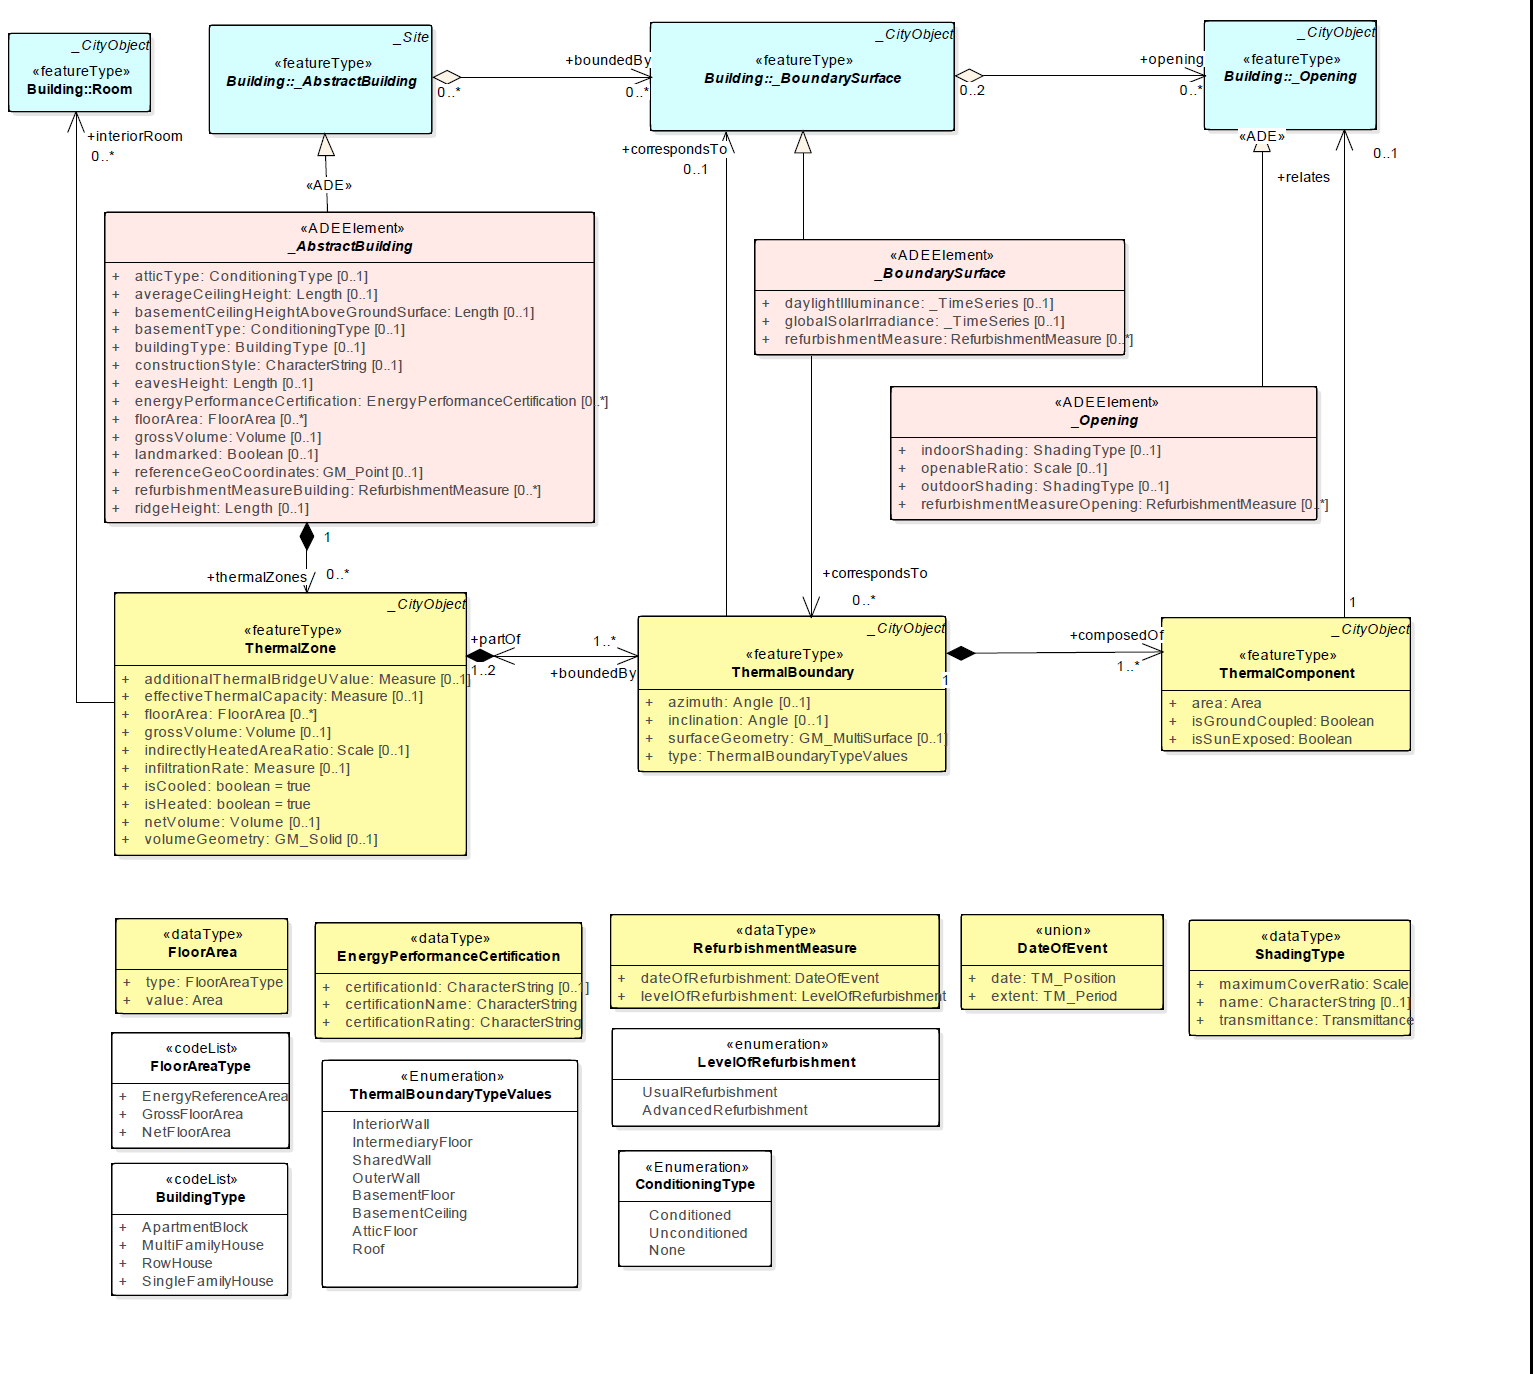
\includegraphics{fig/class_geometry.png}
\caption{Class diagram of Building Physics Module}
\end{figure}

This module contains the thermal building objects required for building
thermal modelling (e.g.~calculation of space heating and space cooling
demands): \lstinline!ThermalZone!, \lstinline!ThermalBoundary!,
\lstinline!ThermalComponent!. These thermal building objects are linked
to the CityGML building objects through its
\lstinline!_AbstractBuilding!, \lstinline!_BoundarySurface!,
\lstinline!_Opening! classes, which are extended with Energy ADE
attributes.

The \lstinline!ThermalZone!, which represents the spatial unit for
heating and cooling demand calculation, is the central object of this
Building Physics Module. A Building may have several
\lstinline!ThermalZone!, for instance in the case of mixed-usage
building, or to distinguish rooms or zones with different solar gains
and/or thermal behaviour.

If occupied, a \lstinline!ThermalZone! must be related to at less 1
\lstinline!UsageZone!, which contains the usage boundary conditions for
the heating and cooling demand calculation (see Occupancy Module).
\lstinline!ThermalZone! may be related to several \lstinline!UsageZone!
for simplified modelling of mixed-usage space, in which case the usage
boundary conditions of the \lstinline!UsageZone! should be aggregated or
weighted according with their floorArea.

These \lstinline!ThermalZone! objects are separated from each other and
from the outside by \lstinline!ThermalBoundary! objects. These
\lstinline!ThermalBoundary! objects may or not correspond to the CityGML
\lstinline!_BoundarySurface!. However, every \lstinline!ThermalBoundary!
delimiting the \lstinline!ThermalZone! from outside must be related
(\lstinline!correspondsTo!) with a \lstinline!_BoundarySurface!, in
order to consider the \lstinline!globalSolarIrradiance! incident on
\lstinline!_BoundarySurface! in the heating and cooling calculations.

\subsection{Extension of CityGML building
objects}\label{extension-of-citygml-building-objects}

\subsubsection{\_AbstractBuilding}\label{abstractbuilding}

The Energy ADE extends the CityGML \_AbstractBuilding by a number of
energy-related attributes, e.g with regards to the geometrical
characteristics (\lstinline!referencePoint!,
\lstinline!averageCeilingHeight!, \lstinline!eavesHeight!,
\lstinline!ridgeHeight!,
\lstinline!basementCeilingHeightAboveGrounSurface!,
\lstinline!floorArea!, \lstinline!grossVolume!), to the conditioning of
basement and attic (\lstinline!basementType!, \lstinline!atticType!), to
the available energy certificates
(\lstinline!energyPerformanceCertification!) and refurbishment measures
(\lstinline!RefurbishmentMeasureOnBuilding!), and other building
information useful for building typology categorisations
(\lstinline!buildingType! and \lstinline!constructionStyle!).

All these attributes are optional. Some of them, like
\lstinline!floorArea! and\\
\lstinline!energyPerformanceCertification!, have a cardinality
{[}0..*{]} and may consequently be attributed several times to a
building, specifying different values for different
\lstinline!FloorAreaType!, respectively \lstinline!certificationName!.

Finally, because \lstinline!_AbstractBuilding! inherits from
\lstinline!_CityObject!, further objects may be assigned to it, like
\lstinline!EnergyDemand! in particular (see Module Energy and Systems).

In the following, an extract of CityGML file for a building is given,
included some of its Energy ADE attributes.

\begin{lstlisting}[language=XML]
<!--Examples of Building with Energy ADE attributes-->
<bldg:Building gml:id="id_building_1">
 <gml:description>Description of Building 1</gml:description>
 <gml:name>Name of Building 1</gml:name>
 <energy:referencePoint>
  <gml:Point gml:id="id_building_referencepoint_1" srsName="EPSG:31256" srsDimension="3">
   <gml:pos>5 5 0</gml:pos>
  </gml:Point>
 </energy:referencePoint>
 <energy:basementType>Unconditioned</energy:basementType>
 <energy:energyPerformanceCertification>
  <!--Here come the EnergyPerformanceCertification objects (see later) -->
 </energy:energyPerformanceCertification>
 <energy:basementCeilingHeightAboveGroundSurface uom="m">1</energy:basementCeilingHeightAboveGroundSurface>
 <energy:grossVolume uom="m^3">1050</energy:grossVolume>
 <energy:refurbishmentMeasureOnBuilding>
  <energy:RefurbishmentMeasure>
   <!--Here come all attributes of a RefurbishmentMeasure object (omitted here)-->
  </energy:RefurbishmentMeasure>
 </energy:refurbishmentMeasureOnBuilding>
 <energy:averageCeilingHeight uom="m">2.7</energy:averageCeilingHeight>
 <energy:atticType>Conditioned</energy:atticType>
 
 <!--Here may come a list of UsageZone of the building (see Module Occupancy) -->
 
 <energy:ridgeHeight uom="m">10.5</energy:ridgeHeight>
 <energy:landmarked>false</energy:landmarked>
 <energy:floorArea>
  <!--Here come the floorArea objects (see later)-->
 </energy:floorArea>
 <energy:eavesHeight uom="m">8</energy:eavesHeight>
 <energy:constructionStyle>Massive</energy:constructionStyle>
 <energy:buildingType>MultiFamilyHouse</energy:buildingType>
 
 <!--Here follow all ThermalZone objects, each inside a "thermalZones" tag-->
 <energy:thermalZones>
  <energy:ThermalZone gml:id="id_thermalzone_1">
   <!--Here come all attributes of the first ThermalZone (omitted here)-->
  </energy:ThermalZone>
 </energy:thermalZones>
 <energy:thermalZones>
  <energy:ThermalZone gml:id="id_thermalzone_2">
   <!--Here come all attributes of the second ThermalZone (omitted here)-->
  </energy:ThermalZone>
 </energy:thermalZones>
</bldg:Building>
\end{lstlisting}

\paragraph{FloorArea}\label{floorarea}

Buildings (\lstinline!_AbstractBuilding!) and building zones
(\lstinline!ThermalZone! and \lstinline!UsageZone!) may have several
\lstinline!floorArea!, related to several \lstinline!FloorAreaType!
(e.g.~net floor area, gross floor area, energy reference area).

\begin{lstlisting}[language=XML]
<!--Examples of three floor areas-->
<energy:FloorArea>
    <energy:FloorArea>
        <energy:type>GrossFloorArea</energy:type>
        <energy:value uom="m^2">50.0</energy:value>
    </energy:FloorArea>
    <energy:FloorArea>
        <energy:type>NetFloorArea</energy:type>
        <energy:value uom="m^2">40.0</energy:value>
    </energy:FloorArea>
    <energy:FloorArea>
        <energy:type>EnergyReferenceArea</energy:type>
        <energy:value uom="m^2">43.0</energy:value>
    </energy:FloorArea>
</energy:FloorArea>
\end{lstlisting}

\paragraph{EnergyPerformanceCertification}\label{energyperformancecertification}

A building may present several\\
\lstinline!energyPerformanceCertification! related to different
\lstinline!certificationName! (e.g.~PassivHaus, LEED) and/or different
certification dates (specificied by \lstinline!certificationId!).

\begin{lstlisting}[language=XML]
<!--Example of two energy performance certifications-->
<energy:energyPerformanceCertification>
    <energy:EnergyPerformanceCertification>
        <energy:certificationRating>Platinum</energy:certificationRating>
        <energy:certificationName>LEED</energy:certificationName>
        <energy:certificationId>0815</energy:certificationId>
    </energy:EnergyPerformanceCertification>
    <energy:EnergyPerformanceCertification>
        <energy:certificationRating>Passive house</energy:certificationRating>
        <energy:certificationName>EnerPHit</energy:certificationName>
        <energy:certificationId>4756</energy:certificationId>
    </energy:EnergyPerformanceCertification>
</energy:energyPerformanceCertification>
\end{lstlisting}

\paragraph{RefurbishmentMeasure}\label{refurbishmentmeasure}

Energy-efficient refurbishment operations and measures may be indicated
as attribute of \lstinline!_AbstractBuilding!,
\lstinline!_BoundarySurface! and \lstinline!_Opening!. The
\lstinline!RefurbishmentMeasure! object contains two information: the
date and level of refurbishment.

The attribute \lstinline!levelOfRefurbishment! is a codeList whose
elements generally relates to refurbishment measure libraries or to a
building typology categorisation.

The attribute \lstinline!dateOfRefurbishment! is defined by the GML type
\lstinline!DateOfEvent!, and may consequently be specified in different
manners (see the 3 examples below).

\begin{lstlisting}[language=XML]
<!--Example of a Refurbishment Measure on a building with a very vague date ("before June 2010") -->
<energy:refurbishmentMeasureOnBuilding>
    <energy:RefurbishmentMeasure>
        <energy:dateOfRefurbishment>
            <energy:DateOfEvent>
                <energy:instant indeterminatePosition="before">2010-06</energy:instant>
            </energy:DateOfEvent>
        </energy:dateOfRefurbishment>
        <energy:levelOfRefurbishment>UsualRefurbishment</energy:levelOfRefurbishment>
        <gml:description>Refurbishment consisting of an outside insulation of walls etc.</gml:description>
    </energy:RefurbishmentMeasure>
</energy:refurbishmentMeasureOnBuilding>
\end{lstlisting}

\begin{lstlisting}[language=XML]
<!--Example of an advanced Refurbishment Measure in the years 1998 and 1999 -->
<energy:refurbishmentMeasureOnBuilding>
    <energy:RefurbishmentMeasure>
        <energy:dateOfRefurbishment>
            <energy:DateOfEvent>
                <energy:period>
                    <gml:TimePeriod>
                        <gml:beginPosition>1998</gml:beginPosition>
                        <gml:endPosition>2000</gml:endPosition>
                    </gml:TimePeriod>
                </energy:period>
            </energy:DateOfEvent>
        </energy:dateOfRefurbishment>
        <energy:levelOfRefurbishment>AdvancedRefurbishment</energy:levelOfRefurbishment>
    </energy:RefurbishmentMeasure>
</energy:refurbishmentMeasureOnBuilding>
\end{lstlisting}

\begin{lstlisting}[language=XML]
<!--Example of an usual Refurbishment Measure in June 2012 -->
<energy:refurbishmentMeasureOnBuilding>
    <energy:RefurbishmentMeasure>
        <energy:dateOfRefurbishment>
            <energy:DateOfEvent>
                <energy:instant>2012-06</energy:instant>
            </energy:DateOfEvent>
        </energy:dateOfRefurbishment>
        <energy:levelOfRefurbishment>UsualRefurbishment</energy:levelOfRefurbishment>
    </energy:RefurbishmentMeasure>
</energy:refurbishmentMeasureOnBuilding>
\end{lstlisting}

\subsubsection{\_Opening}\label{opening}

The CityGML abstract class \lstinline!_Opening! (inherited by the
objects \lstinline!Window! and \lstinline!Door!) is extended in this
Energy ADE by a number of energy-related attributes.

First of all, an optional attribute \lstinline!openableRatio! details
the proportion of the opening area which may be opened. An indoor and an
outdoor shading system may complement the opening, with a
\lstinline!ShadingType! characterized by a \lstinline!transmittance!
(see details in Module Materials and Constructions) and a
\lstinline!maximumCoverRatio!. Finally, information about possible
refurbishment measures and operations may also be added at the level of
the opening (e.g window exchange), through the attribute
\lstinline!refurbishmentMeasureOnOpening! of type
\lstinline!RefurbishmentMeasure!.

As in the Building example shown before, the standard CityGML attributes
have been omitted for better readability. The door example is simpler
and contains also information about construction and construction
orientation (by means of Xlinks).

\begin{lstlisting}[language=XML]
<!--Example of a Window object -->
<bldg:Window gml:id="id_window_1">
    <gml:description>This is window with an outside rolling shutter and curtains inside</gml:description>
    <gml:name>Window with rolling shutter and curtains</gml:name>

    <energy:outdoorShading>
        <energy:ShadingType>
            <energy:maximumCoverRatio uom="ratio">1</energy:maximumCoverRatio>
            <energy:name>Rolling shutter</energy:name>
            <energy:transmittance>
                <energy:Transmittance>
                    <energy:fraction uom="ratio">0</energy:fraction>
                    <energy:wavelengthRange>Total</energy:wavelengthRange>
                </energy:Transmittance>
            </energy:transmittance>
        </energy:ShadingType>
    </energy:outdoorShading>

    <energy:indoorShading>
        <energy:ShadingType>
            <energy:maximumCoverRatio uom="ratio">0.5</energy:maximumCoverRatio>
            <energy:name>Curtain</energy:name>
            <energy:transmittance>
                <energy:Transmittance>
                    <energy:fraction uom="ratio">0.8</energy:fraction>
                    <energy:wavelengthRange>Total</energy:wavelengthRange>
                </energy:Transmittance>
            </energy:transmittance>
        </energy:ShadingType>
    </energy:indoorShading>

    <energy:openableRatio uom="ratio">0.9</energy:openableRatio>

</bldg:Window>
\end{lstlisting}

\subsubsection{\_BoundarySurface, globalSolarIrradiance and
daylightIlluminance}\label{boundarysurface-globalsolarirradiance-and-daylightilluminance}

The CityGML abstract class \lstinline!_BoundarySurface! is extended by a
number of Energy ADE attributes, in order in particular to store the
incident global solar irradiances and the daylight illuminances
available on each outside boundary surface of the building. Moreover,
information about refurbishment measures on roof or facade can
characterised the \lstinline!_BoundarySurface! objects, in the same way
that the buildings and openings, through the attribute
\lstinline!refurbishmentMeasureOnBoundarySurface! of type
\lstinline!RefurbishmentMeasure!.

The \lstinline!globalSolarIrradiance! is the sum of the direct, diffuse
and reflected irradiance incident on a outside boundary surface and is
generally expressed in Watts per square metre. These global solar
irradiance is generally used for the thermal calculations within the
buildings, but also for the calculation of the energy yield produced by
the solar systems (e.g.~photovoltaic and solar thermal panels).

The \lstinline!daylightIlluminance! is the sum of the direct, diffuse
and reflected solar illuminance incident on a outside boundary surface.
It is generally expressed in Lux. Daylight illuminance is typically used
for outside and inside daylighting study, as well as the calculation of
the energy consumptions of lighting systems required to reach the room
illuminance threshold when the daylight illuminance is not enough.

Both \lstinline!globalSolarIrradiance! and
\lstinline!daylightIlluminance! attributes are \lstinline!_Timeseries!
data (see details in Temporal Data Module). In the following, a XML
example of a roof is given.

\begin{lstlisting}[language=XML]
<!--Example of a Roof object -->
<bldg:RoofSurface gml:id="id_roof_1">
    <gml:description>Description of Roof 1</gml:description>
    <gml:name>Name of Roof 1</gml:name>

    <energy:refurbishmentMeasureOnBoundarySurface>
        <energy:RefurbishmentMeasure>
            <!--Here come all attributes of a RefurbishmentMeasure object (omitted here)-->
        </energy:RefurbishmentMeasure>
    </energy:refurbishmentMeasureOnBoundarySurface>

    <energy:globalSolarIrradiance>
        <!--Add here the TimeSeries data -->
    </energy:globalSolarIrradiance>

    <energy:daylightIlliminance>
        <!--Add here the TimeSeries data -->
    </energy:daylightIlliminance>

</bldg:RoofSurface>
\end{lstlisting}

\subsection{Thermal zones, thermal boundaries and thermal
components}\label{thermal-zones-thermal-boundaries-and-thermal-components}

\subsubsection{ThermalZone}\label{thermalzone}

The \lstinline!ThermalZone! is a new object introduced in the Energy ADE
to realize building heating and cooling demand calculation. A
\lstinline!ThermalZone! is a zone of a \lstinline!Building! (or of a
\lstinline!BuildingPart!) which serves as the smallest spatial zone for
building heating and cooling demand calculation. It is generally a
``thermal homogeneous'' space considered as isothermal, but may also
refer to several building rooms and zones with different usage boundary
conditions for simplified building energy modelling.

A \lstinline!ThermalZone! contains a series of energy-related attributes
which characterize its geometry (\lstinline!floorArea!,
\lstinline!grossVolume!, \lstinline!netVolume!,
\lstinline!volumeGeometry!), its conditioning status
(\lstinline!isCooled!, \lstinline!isHeated!,
\lstinline!indirectlyHeatedAreaRatio!) and overall building physics
properties (\lstinline!additionalThermalBridgeUValue!,
\lstinline!infiltration rate!, \lstinline!effectiveThermalCapacity!).

All these attributes are optional. Among those, \lstinline!floorArea!
may be attributed several times to a building, specifying different
values for different \lstinline!FloorAreaType!. A
\lstinline!ThermalZone! may optionally contain an explicit volume
geometry (specified by \lstinline!volumeGeometry!), useful in particular
for visualisation purposes, but not necessary for heating and cooling
demand calculations. The \lstinline!ThermalZone! may also be related to
a room (\lstinline!gml:Room!). The actual surface boundaries of a
\lstinline!ThermalZone! are defined by means of
\lstinline!ThermalBoudary! objects (see later).

If occupied, a \lstinline!ThermalZone! must be related to at less one
\lstinline!UsageZone! object (see Occupancy Module), which contains the
usage boundary conditions for the heating and cooling demand calculation
(see Occupancy Module). \lstinline!ThermalZone! may even be related to
several \lstinline!UsageZone! for simplified modelling of mixed-usage
space, in which case the usage boundary conditions of the UsageZone
should be aggregated or weighted according with their
\lstinline!floorArea!.

The class \lstinline!ThermalZone! inherits from \lstinline!_CityObject!,
and may therefore be associated to one or more \lstinline!EnergyDemand!
objects (see module Energy Systems).

In the following, Two XML examples present a \lstinline!ThermalZone!,
with and without explicit volume geometry.

\begin{lstlisting}[language=XML]
<!--Example of a ThermalZone without explicit volume geometry-->
<energy:ThermalZone gml:id="id_thermalzone_1">
    <gml:description>Description of Thermal Zone 1</gml:description>
    <gml:name>Name of Thermal Zone 1</gml:name>
    <energy:additionalThermalBridgeUValue uom="W/(K*m^2)">0.5</energy:additionalThermalBridgeUValue>
    <energy:effectiveThermalCapacity uom="J/K">500</energy:effectiveThermalCapacity>
    <energy:floorArea>
        <energy:FloorArea>
            <energy:type>EnergyReferenceArea</energy:type>
            <energy:value uom="m^2">55.0</energy:value>
        </energy:FloorArea>
    </energy:floorArea>
    <energy:grossVolume uom="m^3">200.0</energy:grossVolume>

    <!-- here follows a related usage zone -->
    <energy:relates xlink:href="#id_usagezone_1"/>

    <energy:indirectlyHeatedAreaRatio uom="ratio">0.15</energy:indirectlyHeatedAreaRatio>
    <energy:infiltrationRate uom="1/h">1.2</energy:infiltrationRate>
    <energy:isCooled>true</energy:isCooled>
    <energy:isHeated>true</energy:isHeated>
    <energy:netVolume uom="m^3">180.0</energy:netVolume>

    <!--Here follow all ThermalBoundary objects, each inside a "boundedBy" tag-->
    <energy:boundedBy>
        <energy:ThermalBoundary gml:id="id_thermalboundary_1">
            <!--Here come all attributes of the first ThermalBoundary (omitted here)-->
        </energy:ThermalBoundary>
    </energy:boundedBy>
    <energy:boundedBy>
        <energy:ThermalBoundary gml:id="id_thermalboundary_2">
            <!--Here come all attributes of the second ThermalBoundary (omitted here)-->
        </energy:ThermalBoundary>
    </energy:boundedBy>

</energy:ThermalZone>
\end{lstlisting}

\begin{lstlisting}[language=XML]
<!--Example of a ThermalZone with explicit volume geometry-->
<energy:ThermalZone gml:id="id_thermalzone_2">
    <!--Additional attributes of the ThermalZone (omitted here)-->

    <energy:volumeGeometry>
        <gml:Solid gml:id="id_thermalzone_volume_geometry_1" srsName="EPSG:31256" srsDimension="3">
            <gml:exterior>
                <gml:CompositeSurface>
                    <gml:surfaceMember>
                        <gml:Polygon>
                            <gml:exterior>
                                <gml:LinearRing>
                                    <gml:posList>0 0 0 0 10 0 5 10 0 5 0 0 0 0 0</gml:posList>
                                </gml:LinearRing>
                            </gml:exterior>
                        </gml:Polygon>
                    </gml:surfaceMember>
                    <gml:surfaceMember>
                        <gml:Polygon>
                            <gml:exterior>
                                <gml:LinearRing>
                                    <gml:posList>0 0 4 5 0 4 5 10 4 0 10 4 0 0 4</gml:posList>
                                </gml:LinearRing>
                            </gml:exterior>
                        </gml:Polygon>
                    </gml:surfaceMember>
                    <!--Here come further surfaceMember objects-->
                    </gml:CompositeSurface>
            </gml:exterior>
        </gml:Solid>
    </energy:volumeGeometry>
</energy:ThermalZone>
\end{lstlisting}

\subsubsection{ThermalBoundary}\label{thermalboundary}

A \lstinline!ThermalBoundary! represent the physical relationship
between two \lstinline!ThermalZone!, or one \lstinline!ThermalZone! and
the building environment. Its geometrical representation is a coplanar,
or quasi coplanar, surface.

Each \lstinline!ThermalZone! is geometrically closed by its whole set of
bounding \lstinline!ThermalBoundary! (specificied in the relationship
``boundedBy'').

In the case where the \lstinline!ThermalBoundary! delimits one
\lstinline!ThermalZone! from the building environment, corresponding
then to the external boundary of a building, its geometrical
representation coincides with the external surfaces of the related outer
wall/roof/basement floor. In this case, the \lstinline!ThermalBoundary!
should be linked to the corresponding \lstinline!_BoundarySurface!
object (e.g.~a \lstinline!WallSurface!, a \lstinline!RoofSurface!, a
\lstinline!GroundSurface! in LoD2) if existing, through the relationship
``correspondsTo''. It may however occurs that such
\lstinline!ThermalBoundary! does not match with any
\lstinline!_BoundarySurface! (e.g.~basement ceiling, attic floor).

In the case where the \lstinline!ThermalBoundary! separate two adjacent
\lstinline!ThermalZone!, corresponding then to an intermediate floor,
ceiling, or a shared wall, its geometrical representation coincides with
the plan laying at the middle of this construction thickness.

The following figure represents these 2 different cases in a building
side section, relating the Energy ADE objects \lstinline!ThermalZone!
and \lstinline!ThermalBoundary! to the CityGML objects \lstinline!Room!
and \lstinline!_BoundarySurface!.

\begin{figure}[htbp]
\centering
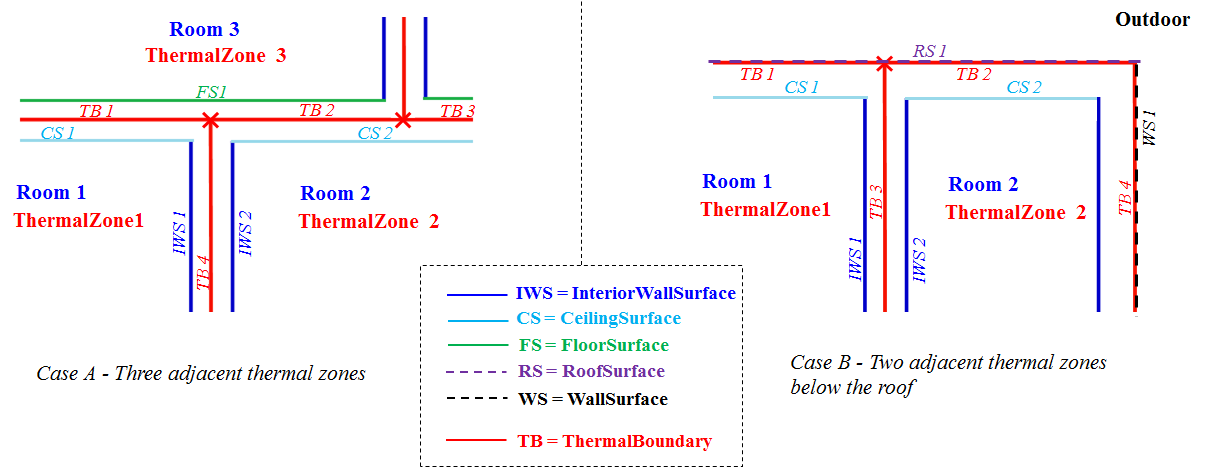
\includegraphics{fig/ThermalZoneAdjacency.png}
\caption{Schema of adjacent thermal zones}
\end{figure}

\lstinline!ThermalBoundary! may contain attributes characterizing their
type\\
(\lstinline!thermalBoundaryType!), orientation (\lstinline!azimuth! and
\lstinline!inclination!) and explicit geometry
(\lstinline!surfaceGeometry!). All these attributes are optional. Thus,
a \lstinline!ThermalZone! may optionally contain an explicit surface
geometry (specified by \lstinline!surfaceGeometry!), useful in
particular for visualisation purposes if the \lstinline!ThermalBoundary!
does not coincide with any \lstinline!_BoundarySurface!, but not
necessary for heating and cooling demand calculations.

The \lstinline!ThermalBoundaryType! type is slightly different to the
types of \lstinline!_BoundarySurface! from CityGML, integrating further
thermal boundaries like AtticFloor, BasementCeiling, BasementFloor or
SharedWall.

Each \lstinline!ThermalBoundaryType! is composed of
\lstinline!ThermalComponent! (e.g.~wall construction, windows etc.)
which holds the \lstinline!Construction!.

In the following, two XML examples of \lstinline!ThermalBoundary!, with
and without explicit geometry are given.

\begin{lstlisting}[language=XML]
<!--Example of a ThermalBoundary corresponding to a building roof, delimiting a thermal zone -->
<energy:ThermalBoundary gml:id="id_thermalboundary_1">
    <gml:description>Thermal Boundary 1</gml:description>
    <gml:name>Thermal Boundary 1</gml:name>
    <energy:azimuth uom="decimal degrees">135</energy:azimuth>
    <energy:inclination uom="decimal degrees">55</energy:inclination>
    <energy:thermalBoundaryType>Roof</energy:thermalBoundaryType>
    <partOf xlink:href="#id_thermalzone_1"/>
    <energy:composedOf>
        <energy:ThermalComponent gml:id="id_thermalcomponent_1">
            <!--Here come all attributes of the first ThermalComponent (omitted here)-->
        </energy:ThermalComponent>
    </energy:composedOf>
    <energy:composedOf>
        <energy:ThermalComponent gml:id="id_thermalcomponent_2">
            <!--Here come all attributes of the second ThermalComponent (omitted here)-->
        </energy:ThermalComponent>
    </energy:composedOf>
    <correspondsTo xlink:href="#id_RoofSurface_1"/>
</energy:ThermalBoundary>
\end{lstlisting}

\begin{lstlisting}[language=XML]
<!--Example of a ThermalBoundary with explicit surface geometry, separating two thermal zones -->
<energy:ThermalBoundary gml:id="id_thermalboundary_2">
    <!--Additional attributes of the ThermalBoundary class (omitted here)-->

    <energy:surfaceGeometry>
        <gml:MultiSurface gml:id="id_thermalboundary_2_surface_geometry" srsName="EPSG:31256" srsDimension="3">
            <gml:surfaceMember>
                <gml:Polygon>
                    <gml:exterior>
                        <gml:LinearRing>
                            <gml:posList>0 0 0 0 10 0 5 10 0 5 0 0 0 0 0</gml:posList>
                        </gml:LinearRing>
                    </gml:exterior>
                </gml:Polygon>
            </gml:surfaceMember>
        </gml:MultiSurface>
    </energy:surfaceGeometry>
    <partOf xlink:href="#id_thermalzone_1"/>
    <partOf xlink:href="#id_thermalzone_2"/>
</energy:ThermalBoundary>
\end{lstlisting}

\subsubsection{ThermalComponent}\label{thermalcomponent}

A \lstinline!ThermalComponent! object is a part of the thermal boundary
corresponding to a homogeneous construction component (e.g.~windows,
wall, insulated part of a wall etc.). Each \lstinline!ThermalComponent!
is characterized with their \lstinline!Area!, information whether it is
coupled to ground (\lstinline!isGroundCoupled!) and exposed to sun
(\lstinline!isSunExposed!).

Since \lstinline!ThermalComponent! inherits from
\lstinline!_CityObject!, it can be associated to a
\lstinline!Construction! object (see module Construction and Material).
This may be done either inline or by means of xlinks (see example
below). In this way, \lstinline!ThermalComponent! provides the physical
properties of the building envelope to calculate the heating and cooling
demand.

\begin{lstlisting}[language=XML]
<!--Example of a ThermalComponent-->
<energy:ThermalComponent gml:id="id_thermalcomponent_1">
    <gml:description>Thermal Component 1</gml:description>
    <gml:name>Thermal Component 1</gml:name>
    <energy:construction xlink:href="#id_construction_1"/>
    <energy:area uom="m^2">50.0</energy:area>
    <energy:isGroundCoupled>false</energy:isGroundCoupled>
    <energy:isSunExposed>true</energy:isSunExposed>
</energy:ThermalComponent>
\end{lstlisting}

\section{Temporal Data Module}\label{temporal-data-module}

This module introduces the two new types \lstinline!_TimeSeries! and
\lstinline!_Schedules!, essential to model the time-depending inputs and
results of urban energy analyses. These types are used in other Modules
of the Energy ADE, in particular the module Occupancy and module Energy
and Systems.

As theses types are actually not domain-specific, we are collaborating
with the development team of the CityGML 3.0 to integrate them in the
new CityGML 3.0 to come (as Dynamizer).

\subsection{Time Series}\label{time-series}

\begin{figure}[htbp]
\centering
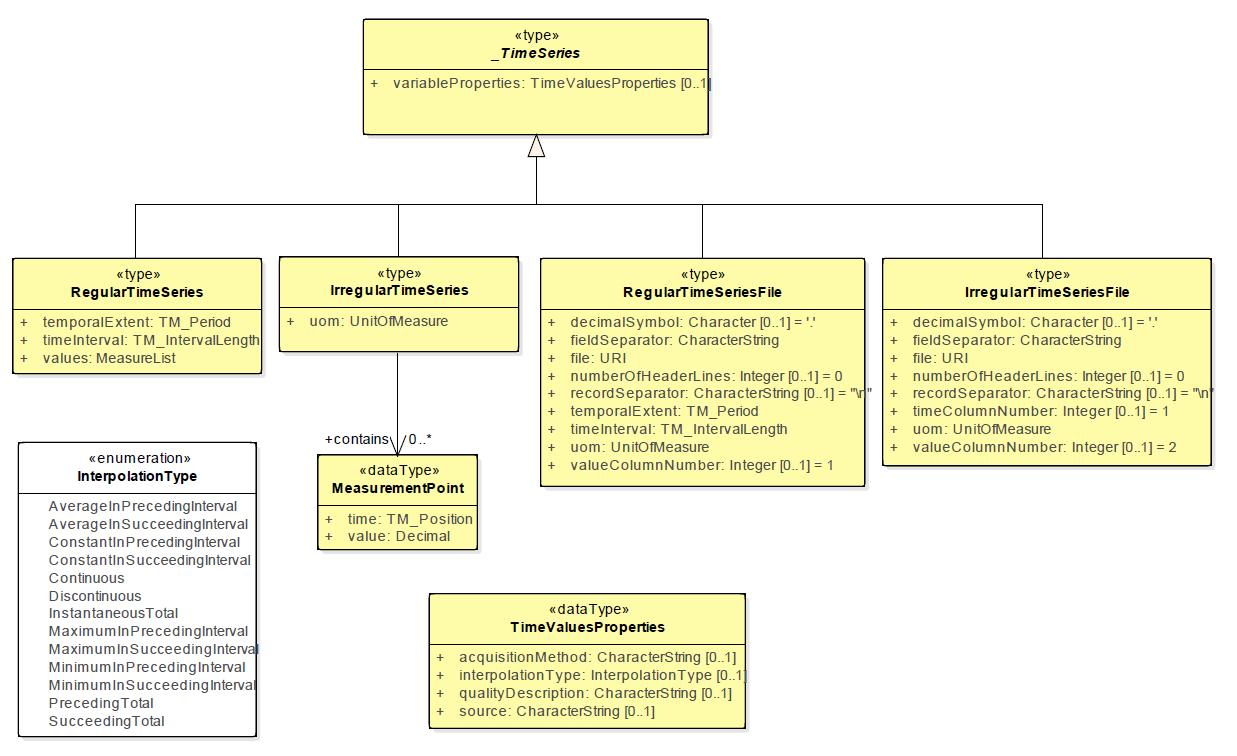
\includegraphics{fig/class_time.png}
\caption{Class diagram of ADE Energy Core - Time Series}
\end{figure}

Time series are homogeneous lists of time-depending values. They are
used in the Energy ADE to store energy amount or an occupancy schedule,
for instance.

All time series share some common properties, gathered in the
\lstinline!TimeValuesProperties! type object. This object specifies
optionally the \lstinline!acquisitionMethod! (e.g.~simulated with
software X, measured with heat meter), \lstinline!interpolationType!
(based on the
\href{http://def.seegrid.csiro.au/sissvoc/ogc-def/resource?uri=http://www.opengis.net/def/waterml/2.0/interpolationType/}{WaterML
ADE} to know for instance if measured data are ``Average in Preceding
Interval'', or ``Instantaneous Total''), \lstinline!qualityDescription!
and \lstinline!source! of the time series data. Additionally,
\lstinline!_TimeSeries!may contain the the usual GML type attributes
\lstinline!name! and \lstinline!description!.

Time series can be either regular or irregular.
\lstinline!RegularTimeSeries! contain \lstinline!values! generated at
regularly spaced interval of time (\lstinline!timeInterval!), over a
given \lstinline!temporalExtent! (i.e.~start, end and duration time).
They are used, for instance, to store automatically acquired data or
hourly/daily/monthly simulation results. In
\lstinline!IrregularTimeSeries!, data follows a temporal sequence, but
the measurement points may not happen at a regular time interval
(\href{http://www-01.ibm.com/support/knowledgecenter/SSCRJU_3.0.0/com.ibm.swg.im.infosphere.streams.timeseries-toolkit.doc/doc/timeseries-regular.html}{IBM
knowledge Center}). Therefore, each value must be associated with a data
or time.

Time series values may be also stored on an external file (e.g.~csv or
text), both for regular (\lstinline!RegularTimeSeriesFile!) and
irregular time series (\lstinline!IrregularTimeSeriesFile!). A number of
attributes must be detailed to retrieve the \lstinline!file!, interprete
the formats and values inside it (\lstinline!decimalSymbol!,
\lstinline!recordSeparator!, \lstinline!fieldSeparator!,
\lstinline!numberOfHeaderLines!, \lstinline!uom!), and know which values
of the file should be read (\lstinline!timeColumnNumber! for irregular
time series and \lstinline!valueColumnNumber! for both of them). One
file with different records may be reused by different
\lstinline!RegularTimeSeriesFile! or \lstinline!IrregularTimeSeriesFile!
with the corresponding \lstinline!valueColumnNumber!.

In the following, four examples of time series illustrates the four
types of time series. The variableProperties and gml attributes are
presented in the first example but not always repeated in the following
examples for better readibility.

Example of RegularTimeSeries object:

\begin{lstlisting}[language=XML]
<!--Example of RegularTimeSeries object with daily values-->
<energy:RegularTimeSeries gml:id="id_timeseries_electricity_demand_1">
    <gml:description>Description of the time series id_timeseries_electricity_demand_1</gml:description>
    <gml:name>Name of the  time series id_timeseries_electricity_demand_1</gml:name>
    <energy:variableProperties>
        <energy:TimeValuesProperties>
            <energy:acquisitionMethod>Measured electronically with heat power</energy:acquisitionMethod>
            <energy:interpolationType>AverageInSucceedingInterval</energy:interpolationType>
            <energy:qualityDescription>Accurate (+/- 0.2 kWh)</energy:qualityDescription>
            <energy:source>Subcontracting company X</energy:source>
        </energy:TimeValuesProperties>
    </energy:variableProperties>
    <energy:temporalExtent>
        <gml:TimePeriod>
            <gml:beginPosition>2016-01-01</gml:beginPosition>
            <gml:endPosition>2016-12-31</gml:endPosition>
        </gml:TimePeriod>
    </energy:temporalExtent>
    <energy:timeInterval unit="day">1</energy:timeInterval>
    <energy:values uom="kWh">11.2 11.4 10.2 9.6 6.3 11.5 12.7 ... (truncated, set of 365 values) </energy:values>
</energy:RegularTimeSeries>
\end{lstlisting}

Example of IrregularTimeSeries object:

\begin{lstlisting}[language=XML]
<!--Example of IrregularTimeSeries object listing one value per year-->
<energy:IrregularTimeSeries gml:id="id_timeseries_electricity_demand_1">
    <energy:variableProperties>
        <energy:TimeValuesProperties>
            <energy:acquisitionMethod>Manual read on electrical meter</energy:acquisitionMethod>
            <energy:interpolationType>InstantTotal</energy:interpolationType>
        </energy:TimeValuesProperties>
    </energy:variableProperties>
    <energy:uom uom="kWh"/>
    <energy:contains>
        <energy:MeasurementPoint>
            <energy:time>2010-02-24</energy:time>
            <energy:value>12050</energy:value>
        </energy:MeasurementPoint>
    </energy:contains>
    <energy:contains>
        <energy:MeasurementPoint>
            <energy:time>2011-02-15</energy:time>
            <energy:value>14050</energy:value>
        </energy:MeasurementPoint>
    </energy:contains>
    <energy:contains>
        <energy:MeasurementPoint>
            <energy:time>2012-03-01</energy:time>
            <energy:value>16245</energy:value>
        </energy:MeasurementPoint>
    </energy:contains>
</energy:RegularTimeSeries>
\end{lstlisting}

Example of RegularTimeSeriesFile object:

\begin{lstlisting}[language=XML]
<!--Example of RegularTimeSeriesFile object with hourly values contained in a file-->
<energy:RegularTimeSeriesFile gml:id="id_regulartimeseries_file_1">
    <energy:uom uom="W/m^2"/>
    <energy:file>file_name_containing_values.csv</energy:file>
    <energy:temporalExtent>
        <gml:TimePeriod>
            <gml:beginPosition>2008-01-01</gml:beginPosition>
            <gml:endPosition>2008-12-31</gml:endPosition>
        </gml:TimePeriod>
    </energy:temporalExtent>
    <energy:timeInterval unit="hour">1</energy:timeInterval>
    <energy:numberOfHeaderLines>1</energy:numberOfHeaderLines>
    <energy:valueColumnNumber>1</energy:valueColumnNumber>
    <energy:fieldSeparator>\t</energy:fieldSeparator>
</energy:RegularTimeSeriesFile>
\end{lstlisting}

Example of IrregularTimeSeriesFile object:

\begin{lstlisting}[language=XML]
<!--Example of IrregularTimeSeriesFile object-->
<energy:RegularTimeSeriesFile gml:id="id_regulartimeseries_file_1">
    <energy:uom uom="W/m^2"/>
    <energy:file>file_name_containing_values.csv</energy:file>
    <energy:numberOfHeaderLines>1</energy:numberOfHeaderLines>
    <energy:recordSeparator> </energy:recordSeparator>
    <energy:decimalSymbol>,</energy:decimalSymbol>
    <energy:valueColumnNumber>9</energy:valueColumnNumber>
    <energy:timeColumnNumber>1</energy:timeColumnNumber>
    <energy:fieldSeparator>\t</energy:fieldSeparator>
</energy:RegularTimeSeriesFile>
\end{lstlisting}

\subsection{Schedules}\label{schedules}

\begin{figure}[htbp]
\centering
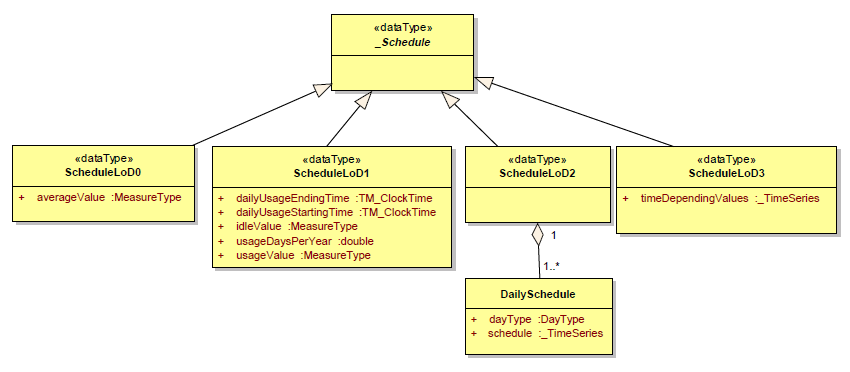
\includegraphics{fig/class_schedules.png}
\caption{Class diagram of ADE Energy Core - Schedules}
\end{figure}

The type \lstinline!_Schedule! is used in the Energy ADE for different
kinds of schedules related to the building usage: heating and cooling
schedules (set-point temperatures), ventilation schedules (mechanical
air change rate), occupancy rate and facilities operation schedules.

Schedules can be modelled in 4 possible ``semantic levels of detail'',
depending on the available information and the application requirements.
These levels of detail range from a simple constant value to a detailed
schedule characterised by a \lstinline!_TimeSeries! object.

\subsubsection{ConstantValueSchedule}\label{constantvalueschedule}

The simplest level of detail, this Schedule is defined by a constant
measure (\lstinline!averageValue!), generally corresponding to the
average parameter value.

\begin{lstlisting}[language=XML]
<!--Example of a ConstantValueSchedule-->
<energy:ConstantValueSchedule gml:id="id_constant_schedule_1">
    <energy:averageValue uom="degree Celsius">26</energy:averageValue>
</energy:ConstantValueSchedule>
\end{lstlisting}

\subsubsection{DualValueSchedule}\label{dualvalueschedule}

A two-state schedule. This schedule is defined by a
\lstinline!usageValue! for usage times, and an \lstinline!idleValue!
outside these temporal boundaries. Usage times are characterized by the
numbers \lstinline!usageHoursPerDay! and \lstinline!usageHoursPerDay!
(usage hours per usage days). This schedule complies in particular with
the data requirements of the codes and norms describing the monthly
energy balance (DIN 18599-2, ISO 13790).

\begin{lstlisting}[language=XML]
<!--Example of a DualValueSchedule-->
<energy:DualValueSchedule gml:id="id_dualvalue_schedule_2">
    <energy:usageValue uom="degree Celsius">20</energy:usageValue>
    <energy:idleValue uom="degree Celsius">16</energy:idleValue>
    <energy:usageHoursPerDay uom="hour">17</energy:usageHoursPerDay>
    <energy:usageDaysPerYear uom="day">365</energy:usageDaysPerYeary>
</energy:DualValueSchedule>
\end{lstlisting}

\subsubsection{DailyPatternSchedule}\label{dailypatternschedule}

This more detailed schedule is composed of daily \lstinline!schedule!
associated to recurrent \lstinline!dayType! (e.g.~weekday, weekend).
These daily schedules are of type\lstinline!_TimeSeries!, as described
above.

\begin{lstlisting}[language=XML]
<!--Example of a daily pattern schedule for a standard week composed of weekday and weekend days-->
<energy:DailyPatternSchedule gml:id="id_dailypattern_schedule_3">
    <energy:dailySchedule>
        <energy:DailySchedule>
            <energy:dayType>WeekDay</energy:dayType>
            <energy:schedule>
                <energy:RegularTimeSeries gml:id="id_occupants_daily_timeseries_1">
                    <energy:temporalExtent>
                        <gml:TimePeriod>
                            <gml:beginPosition>00:00:00</gml:beginPosition>
                            <gml:endPosition>23:59:59</gml:endPosition>
                        </gml:TimePeriod>
                    </energy:temporalExtent>
                    <energy:timeInterval unit="hour">1</energy:timeInterval>
                    <energy:values uom="ratio">0 0 0 0.1 0.2 0.5 ... (truncated, set of 24 values)</energy:values>
                </energy:RegularTimeSeries>
            </energy:schedule>
        </energy:DailySchedule>
    </energy:dailySchedule>
    <energy:dailySchedule>
        <energy:DailySchedule>
            <energy:dayType>WeenEnd</energy:dayType>
            <energy:schedule>
                <energy:RegularTimeSeries gml:id="id_occupants_daily_timeseries2">
                    <energy:temporalExtent>
                        <gml:TimePeriod>
                            <gml:beginPosition>00:00:00</gml:beginPosition>
                            <gml:endPosition>23:59:59</gml:endPosition>
                        </gml:TimePeriod>
                    </energy:temporalExtent>
                    <energy:timeInterval unit="hour">1</energy:timeInterval>
                    <energy:values uom="ratio">0 0 0 0.11 0.22 ... (truncated, set of 24 values)</energy:values>
                </energy:RegularTimeSeries>
            </energy:schedule>
        </energy:DailySchedule>
    </energy:dailySchedule>
</energy:DailyPatternSchedule>
\end{lstlisting}

\subsubsection{TimeSeriesSchedule}\label{timeseriesschedule}

This type is the most detailed of all \lstinline!_schedule! levels of
details. It consists of a unique time series, without patterns.

\begin{lstlisting}[language=XML]
<!--Example of a time series based schedule with hourly values for one year-->
<energy:TimeSeriesSchedule gml:id="id_timeseries_schedule_4">
    <energy:RegularTimeSeries "id_occupants_timeseries4">
            <energy:temporalExtent>
                <gml:TimePeriod>
                    <gml:beginPosition>2000-01-01</gml:beginPosition>
                    <gml:endPosition>2000-12-31</gml:endPosition>
                </gml:TimePeriod>
            </energy:temporalExtent>
            <energy:timeInterval unit="hour">1</energy:timeInterval>
            <energy:values uom="ratio">1 1 1 1 0.9 0.7 0.5 ... (truncated, set of 8760 values)</energy:values>
    </energy:RegularTimeSeries>
</energy:TimeSeriesSchedule>
\end{lstlisting}

\section{Construction and Material
Module}\label{construction-and-material-module}

\begin{figure}[htbp]
\centering
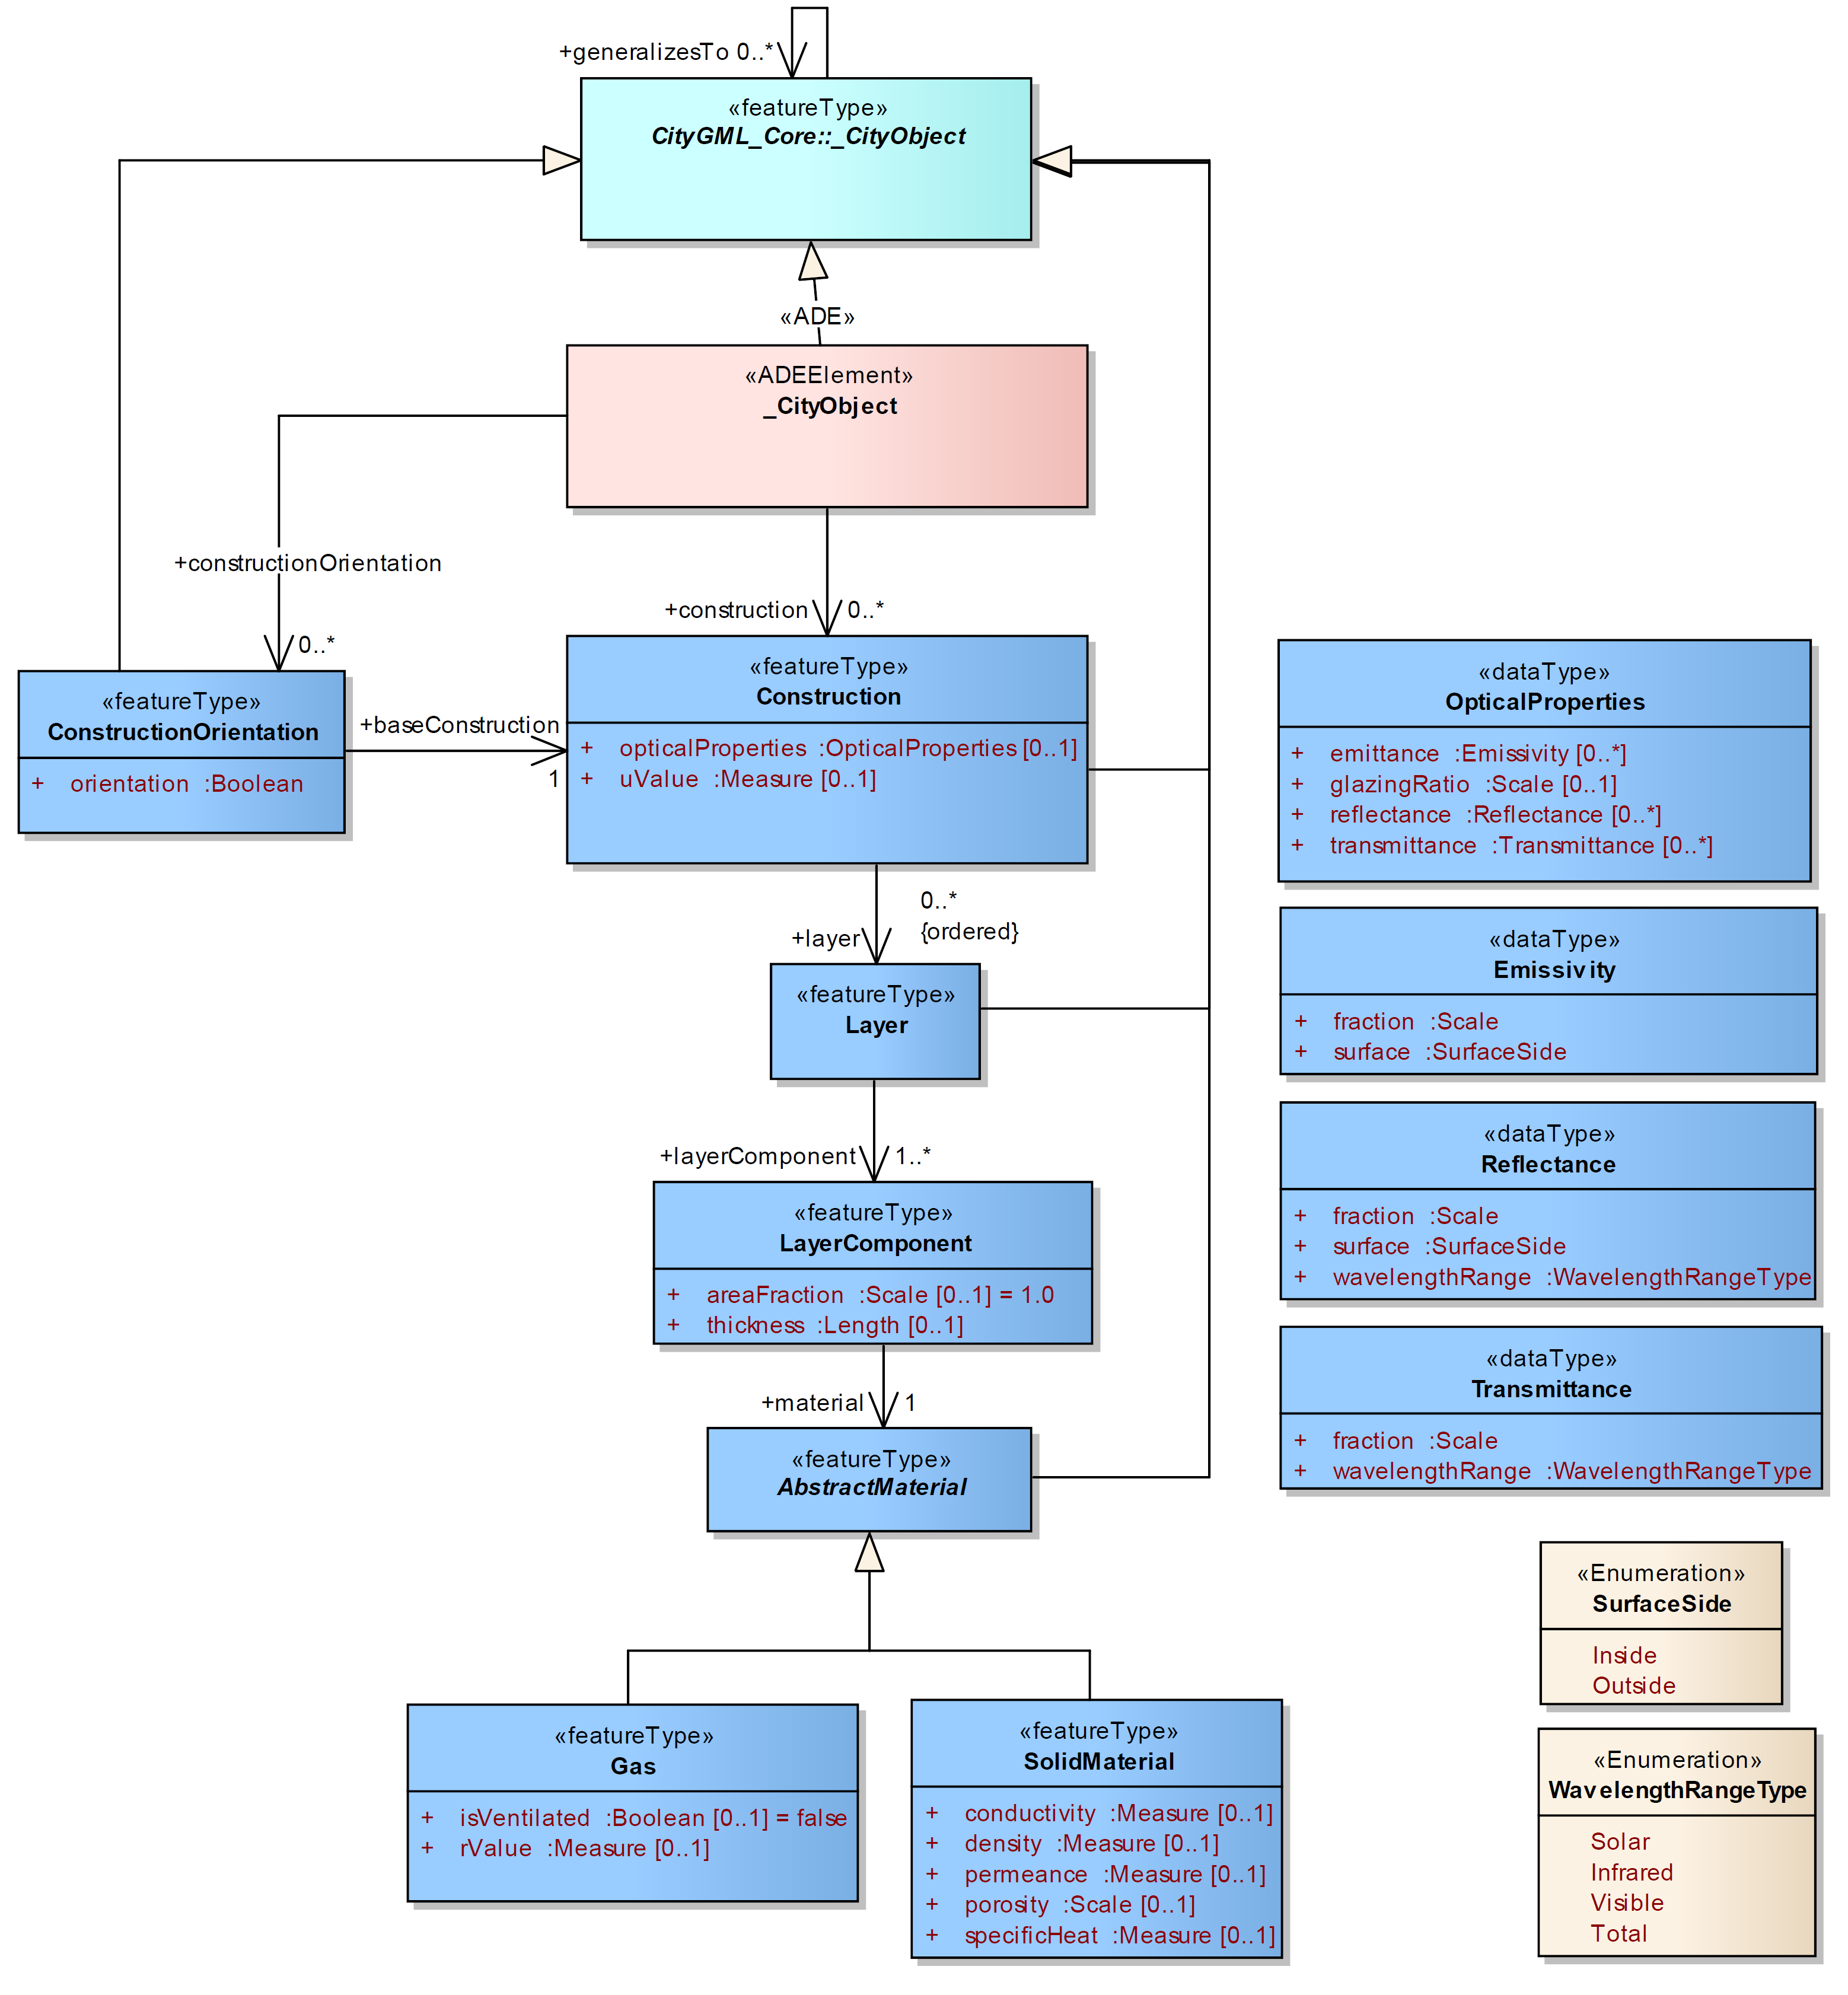
\includegraphics{fig/class_construction.png}
\caption{Class diagram of Construction Module}
\end{figure}

The Construction and Material module of the ADE Energy characterizes
physically the building construction parts, detailing their structure
and specifiying their thermal and optical properties.

As its central object \lstinline!Construction! inherits from class
\lstinline!_CityObject!, all similar objects, can be described by means
of construction and materials.

Given that the nature of this module is not domain-specific, it can be
used beyond energy-related applications (e.g.~in statics, acoustics
etc.)

\subsection{Construction}\label{construction}

This is the central object of this module, which holds the physical
characterisation of building envelop or intern room partition
(e.g.~wall, roof, openings). In the Energy ADE, the object
\lstinline!Construction! is generally linked to the object
\lstinline!ThermalComponents! for space heating and cooling demand
calculations, in order to specified in the building model the physical
parameters of walls, roofs of windows etc. However, it may possibly be
linked to any \lstinline!_CityObject! for other purposes, in particular
to \lstinline!_BoundarySurface!, \lstinline!_Opening! or even
\lstinline!_AbstractBuilding!.

Each \lstinline!Construction! object may be characterised by optical
and/or physical properties.

The \lstinline!OpticalProperties! type specified the
\lstinline!emissivity!, \lstinline!reflectance!,
\lstinline!transmittance! and \lstinline!glazingRatio! of the
construction and its surfaces:

\begin{itemize}
\item
  \emph{Emissivity} is the ratio of the infrared (also called long-wave)
  radiation emitted by a specific surface/object to that of a black
  body. It is specified for a given surface (\lstinline!SurfaceSide!).
  According with the Kirchoff and Lambert law, for a diffuse grey body
  the aborptance and the emittance are equal for a given wavelength
  range.
\item
  \emph{Reflectance} is the fraction of incident radiation which is
  reflected by an object. It is specified for a given surface
  (\lstinline!SurfaceSide!) and for a given \lstinline!wavelengthRange!
  type (``Visible'', ``Infrared'', ``Solar'' or ``Total'' spectrums).
\item
  \emph{Transmittance} is the fraction of incident radiation which
  passes through a specific object. It is specified for a given
  \lstinline!wavelengthRange! type . For example, the total
  transmittance of a window correspond to its \emph{g-value} (also
  called Solar Heat Gain Coefficient). The transmittance value is
  included between 0 (completely opaque object) and 1 (completely
  transparent object).
\item
  the \lstinline!glazingRatio! corresponds of to proportion of the
  construction surface which is transparent and for which the
  transmittance is defined. For the modelling of window,
  \lstinline!glazingRatio! corresponds to the proportion of window
  surface not cover by the window frame.
\end{itemize}

The thermal properties of the Construction may be characterized with two
possible ``levels of details'' : either with the heat transmission
coefficient \lstinline!uValue! for steady-state thermal modelling, or by
detailing its different \lstinline!Layer! of materials and their thermal
behaviour.

In this last case, the \lstinline!Construction! may be defined as an
ordered combination of \lstinline!Layer!, containing possibly several
\lstinline!LayerComponent! made of materials.

In the following, several examples of Construction objects are
presented, with different levels of complexity.

A simple wall characterised with its U-value :

\begin{lstlisting}[language=XML]
<!--Example of a wall construction simply characterised with a U-value-->
<energy:Construction gml:id="id_construction_1">
    <gml:description>Description of Construction 1</gml:description>
    <gml:name>Name of Construction 1</gml:name>
    <energy:uValue uom="W/(K*m^2)">1.2</energy:uValue>
</energy:Construction>
\end{lstlisting}

A window characterised with its U-value, its emissivity, its g-value and
its visible transmittance.

\begin{lstlisting}[language=XML]
<!--Example of low-emissivity window Construction object-->
<energy:Construction gml:id="id_construction_2">
    <gml:description>Description of the windows Construction</gml:description>
    <gml:name>Name of the window Construction</gml:name>
    <energy:uValue uom="W/(K*m^2)">1.9</energy:uValue>
    <energy:opticalProperties>
        <energy:OpticalProperties>
            <energy:emittance>
                <energy:Emissivity>
                    <energy:fraction uom="ratio">0.04</energy:fraction>
                    <energy:surface>Inside</energy:surface>
                </energy:Emissivity>
            </energy:emittance>
            <!-- Here follows the g-value (or SHGC) characterization-->
            <energy:transmittance>
                <energy:Transmittance>
                    <energy:fraction uom="ratio">0.65</energy:fraction>
                    <energy:wavelengthRange>Total</energy:wavelengthRange>
                </energy:Transmittance>
            </energy:transmittance>
            <!-- Here follows the visible transmittance characterization-->
            <energy:transmittance>
                <energy:Transmittance>
                    <energy:fraction uom="ratio">0.55</energy:fraction>
                    <energy:wavelengthRange>Visible</energy:wavelengthRange>
                </energy:Transmittance>
            </energy:transmittance>
            <energy:glazingRatio uom="ratio">0.8</energy:glazingRatio>
        </energy:OpticalProperties>
    </energy:opticalProperties>
</energy:Construction>
\end{lstlisting}

\subsubsection{ConstructionOrientation}\label{constructionorientation}

This class defines the orientation convention of the
\lstinline!Construction! object it is referred to. In other words, it
indicates in which order the layers are to be considered (from inside to
outside, or viceversa), because the same construction, if common to
different zones or buildings, might be orientated in two different
directions for instance.

\begin{lstlisting}[language=XML]
<!--Example of ConstructionOrientation object-->
<energy:ConstructionOrientation gml:id="id_construction_orientation_ground_1">
    <gml:description>Description of Construction Orientation 1 (from inside to outside)</gml:description>
    <gml:name>Name of Construction Orientation 1</gml:name>
    <energy:orientation>true</energy:orientation>
    <energy:baseConstruction xlink:href="#id_construction_1"/>
</energy:ConstructionOrientation>
\end{lstlisting}

\subsection{Layers and layer
components}\label{layers-and-layer-components}

A \lstinline!Construction! may be defined as an ordered combination of
layers, themselves composed of one or more \lstinline!LayerComponent!. A
\lstinline!LayerComponent! is a homogeneous part of a \lstinline!Layer!
(composed of a unique material) covering a given fraction
(\lstinline!areaFraction!) of it.

The materials of each \lstinline!LayerComponent! may be specified either
inline or by means of xlinks (more adapted to materials reused in
different constructions).

The XML example below characterizes a insulated outer wall construction
with three layers. The materials are referenced with xlinks (the
material characterization of ID\_Material\_Concrete follows in the
paragrap Material).

\begin{lstlisting}[language=XML]
<!--Example of a three layered construction-->
<energy:Construction gml:id="ThreeLayeredMaterial">
 <energy:layer>
  <energy:Layer>
   <energy:layerComponent>
    <energy:LayerComponent>
     <energy:thickness uom="m">0.02</energy:thickness>
     <energy:material xlink:href="#ID_Material_Plasterboard"/>
    </energy:LayerComponent>
   </energy:layerComponent>

   <energy:layerComponent>
    <energy:LayerComponent>
     <energy:thickness uom="m">0.24</energy:thickness>
     <energy:material xlink:href="#ID_Material_Concrete"/>
    </energy:LayerComponent>
   </energy:layerComponent>

   <energy:layerComponent>
    <energy:LayerComponent>
     <energy:thickness uom="m">0.12</energy:thickness>
     <energy:material xlink:href="#ID_Material_Polyurethan"/>
    </energy:LayerComponent>
   </energy:layerComponent>
  </energy:Layer>
 </energy:layer>
</energy:Construction>
\end{lstlisting}

{[}Picture: Cut of the wall of the same wall - Joachim? Peter?{]}

\subsection{Materials}\label{materials}

\subsubsection{AbstractMaterial}\label{abstractmaterial}

\lstinline!_AbstractMaterial! is the abstract superclass for all
Material classes. A Material is a homogeneous substance. We distinguish
solid materials (with mass) from gas (without mass).

\subsubsection{SolidMaterial}\label{solidmaterial}

\lstinline!SolidMaterial! is the class of materials which have a mass
and a heat capacity.

\begin{lstlisting}[language=XML]
<!-- Characterisation of the material Concrete-->
<energy:material gml = "ID_Material_Concrete">
        <energy:SolidMaterial>
                <gml:name>Concrete 2100</gml:name>
                <energy:conductivity uom="W/(K*m^2)">2.035</energy:conductivity>
                <energy:density uom="kg/m^3">2100.0</energy:density>
                <energy:specificHeat uom="J/(K*kg)">920.0</energy:specificHeat>
        </energy:SolidMaterial>
</energy:material>
\end{lstlisting}

\subsubsection{Gas}\label{gas}

\lstinline!Gas! is the class of materials whose mass and heat capacity
are neglectable in comparison with \lstinline!SolidMaterial!.

\begin{lstlisting}[language=XML]
<!--Example of a gas material with neglectable mass and heat capacity-->
<energy:material>
    <energy:Gas>
        <gml:name>non-ventilated air gap</gml:name>
        <energy:isVentilated>false</energy:isVentilated>
        <energy:rValue uom="K*m^2/W">4.5</energy:rValue>
    </energy:Gas>
</energy:material>
\end{lstlisting}

\section{Occupancy Module}\label{occupancy-module}

\begin{figure}[htbp]
\centering
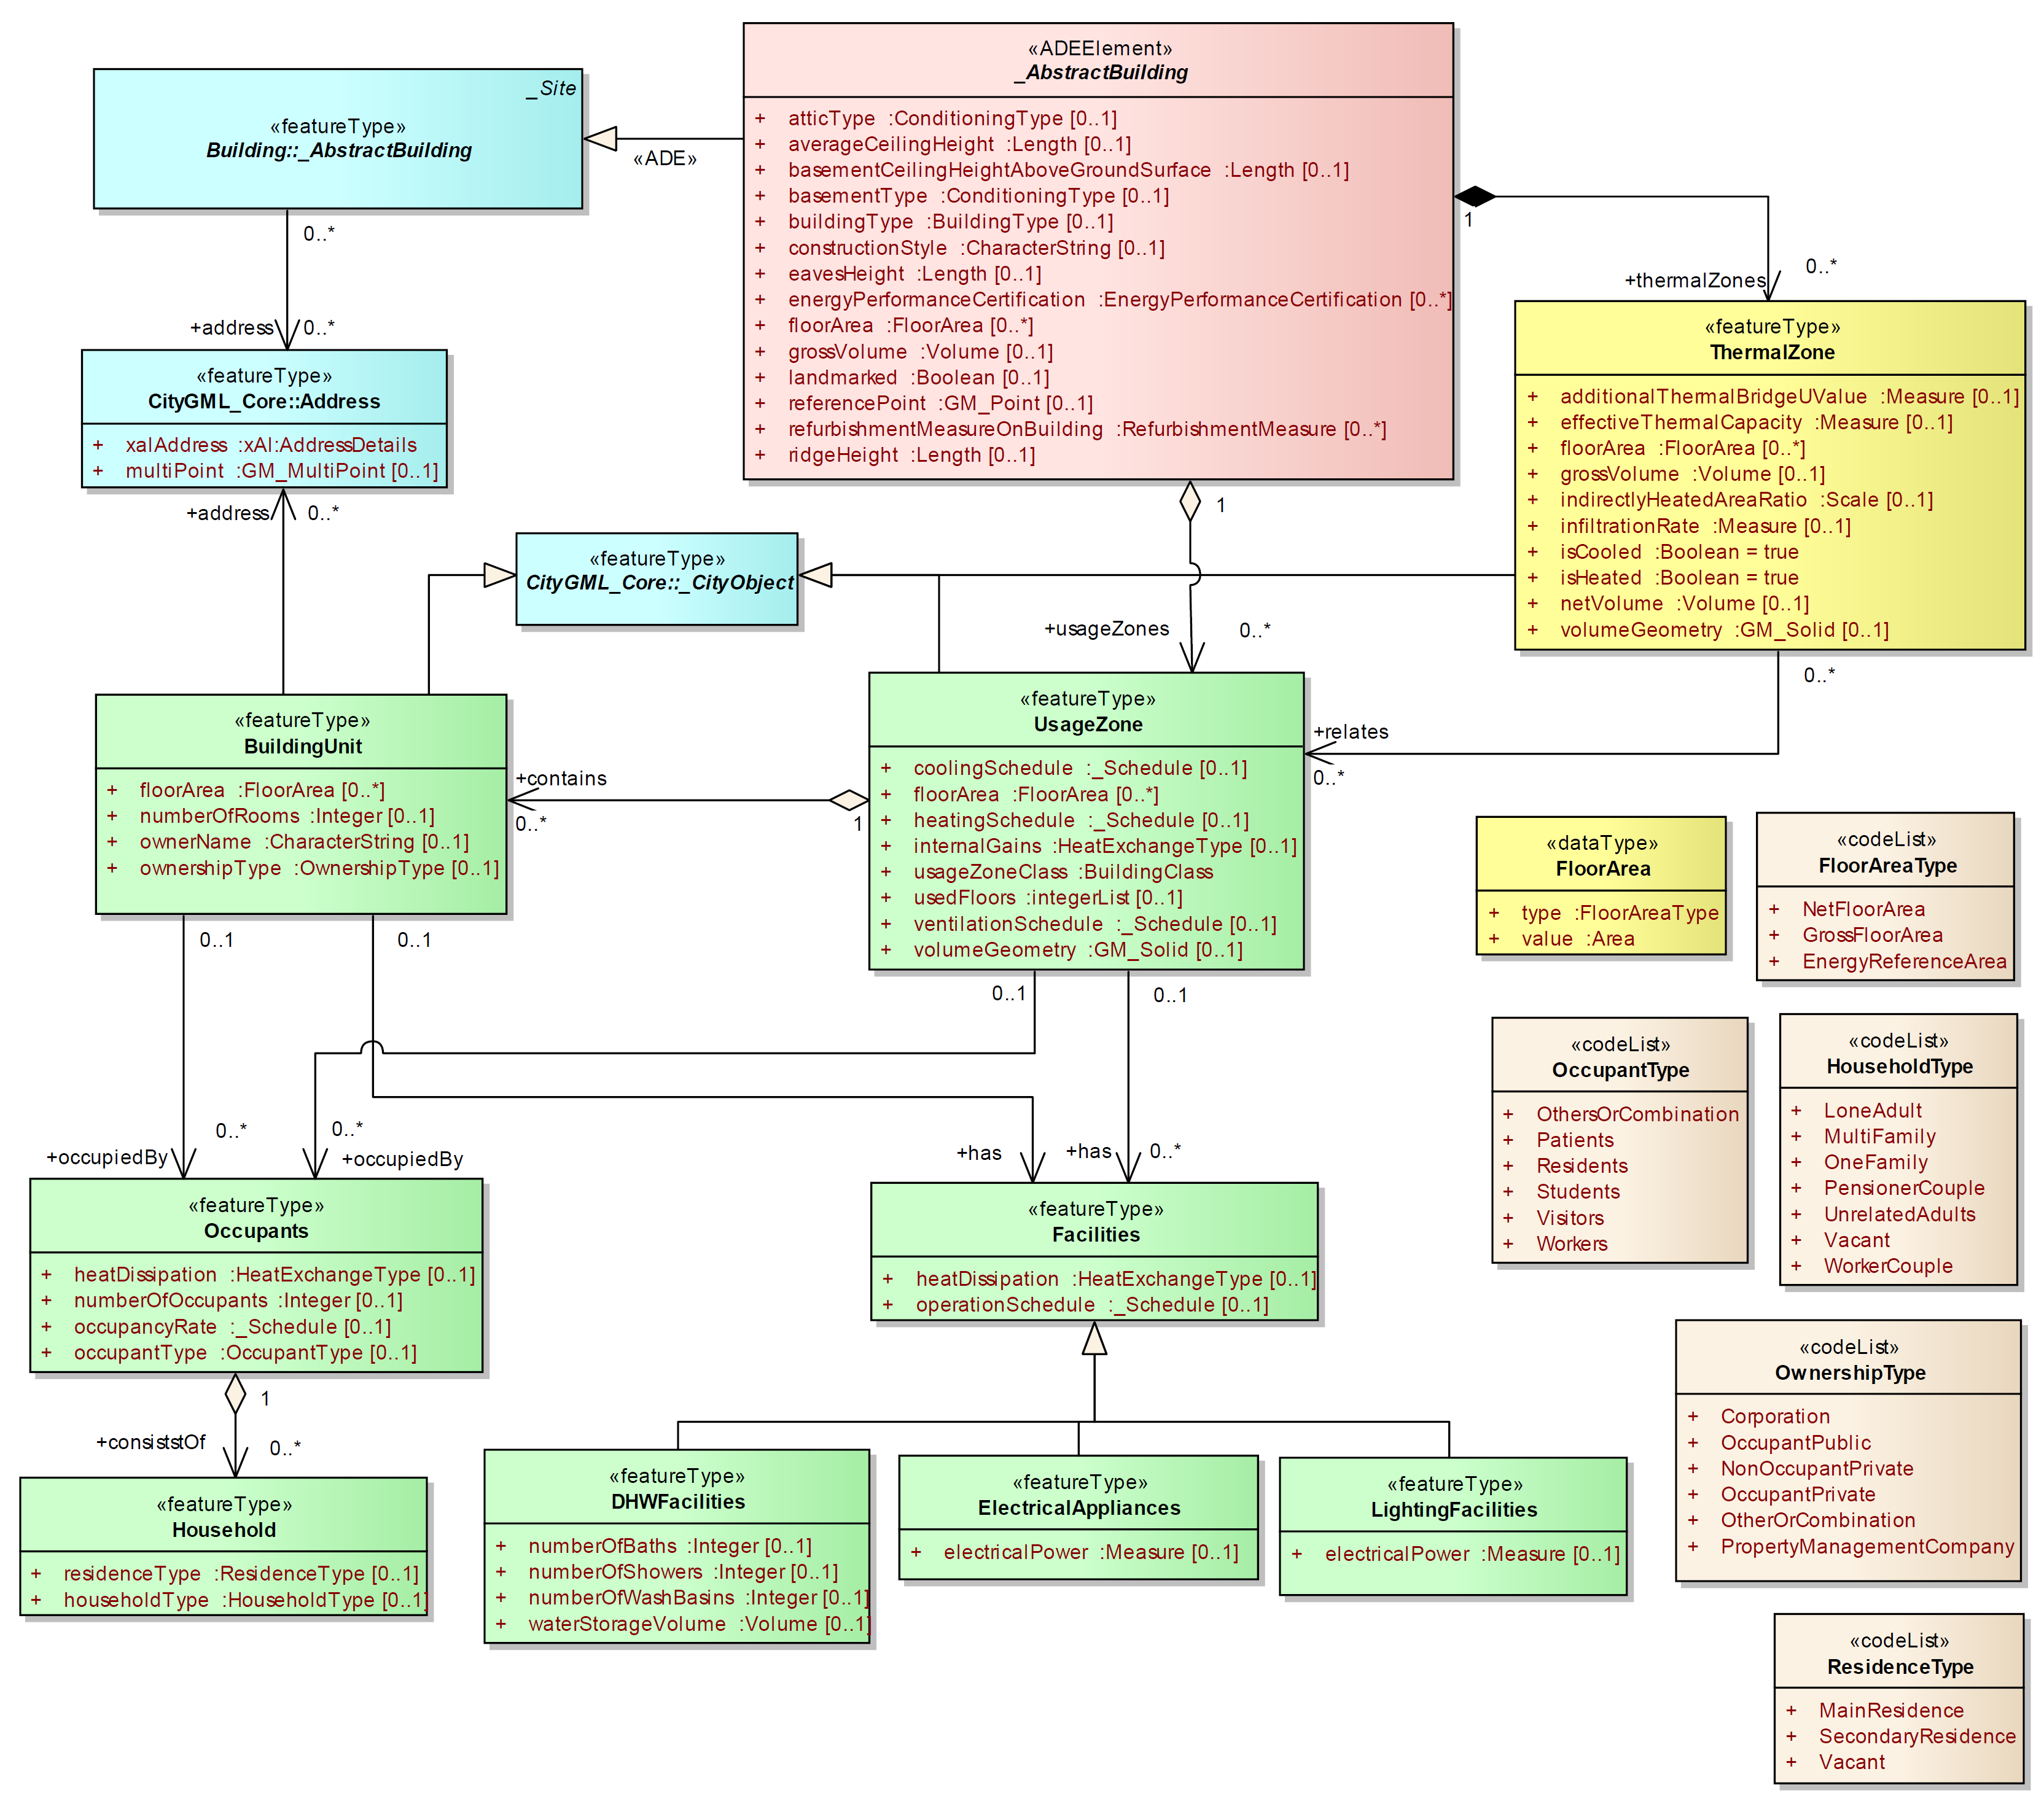
\includegraphics{fig/class_occupancy.png}
\caption{Class diagram of Occupancy Module}
\end{figure}

The Occupancy Module contains the detailed characterization of the
building usage, it is related to the rest of the ADE Energy and CityGML
model through the class \lstinline!UsageZone!. Due to the type of
information it allows to store, the Occupancy Module may be used also
for multi-field analysis (socio-economics, demographics etc.).

\subsection{Usage zones and building
units}\label{usage-zones-and-building-units}

\subsubsection{UsageZone}\label{usagezone}

Zone of a building with homogeneous usage type. It is a semantic object,
with an optional geometry (\lstinline!volumeGeometry!), which may be or
not related to a geometric entity (Building, BuildingPart, Room etc.).

Its usage type is defined by a \lstinline!usageZoneClass! (corresponding
to the CityGML Code list of the \lstinline!_AbstractBuilding! attribute
class). This zone is operated with a single heating and cooling
set-point temperature schedule (\lstinline!heatingSchedule! respectively
\lstinline!coolingSchedule!) and single air ventilation schedule.

This class inherits from \lstinline!_CityObject! and may therefore be
associated to 1 or more \lstinline!EnergyDemand! objects. This class is
defined by at least a usage zone class and a floor area. The building
storeys occupied by this UsageZone may be also indicated by means of the
attribute usedFloorNumbers, e.g.~with 0 corresponding to the ground
floor. Its internalGains attribute corresponds to the sum of the energy
dissipated from the occupants and the facilities inside the zone.

\begin{lstlisting}[language=XML]
<!--Example of a UsageZone-->
<energy:UsageZone gml:id="id_usagezone_1">
    <gml:description>Description of UsageZone 1</gml:description>
    <gml:name>Name of UsageZone 1</gml:name>
    <energy:usageZoneClass>Commercial</energy:usageZoneClass>
    <energy:usedFloors>1</energy:usedFloors>
    <energy:floorArea>
        <energy:FloorArea>
            <energy:type>NetFloorArea</energy:type>
            <energy:value>40</energy:value>
        </energy:FloorArea>
    </energy:floorArea>
    <energy:internalGains>
        <energy:HeatExchangeType>
            <energy:convectiveFraction uom="ratio">0.6</energy:convectiveFraction>
            <energy:latentFraction uom="ratio">0.1</energy:latentFraction>
            <energy:radiantFraction uom="ratio">0.3</energy:radiantFraction>
            <energy:totalValue uom="kW/m^2">80</energy:totalValue>
        </energy:HeatExchangeType>
    </energy:internalGains>

    <!--Here follow all BuildingUnit objects, each inside a "contains" tag-->
    <energy:contains>
        <energy:BuildingUnit gml:id="id_buildingunit_1">
            <!--Here come all attributes of the first BuildingUnit (if needed) -->
        </energy:BuildingUnit>
    </energy:contains>
    <!--Add more BuildingUnit objects here (if needed) -->

    <!--Here follow all Occupants objects, each inside a "occupiedBy" tag-->
    <energy:occupiedBy>
        <energy:Occupants gml:id="id_occupants_1">
            <!--Here come all attributes of the Occupants object -->
        </energy:Occupants>
    </energy:occupiedBy>

    <!--Here follow all Facility objects, each inside a "has" tag-->
    <energy:has>
        <energy:DHWFacilities gml:id="id_dhwfacilities_1">
            <!--Here come all attributes of a Facility object -->
        </energy:ElectricalAppliances>
    </energy:has>
    <energy:has>
        <energy:ElectricalAppliances gml:id="id_electricalappliance_1">
            <!--Here come all attributes of a Facility object -->
        </energy:ElectricalAppliances>
    </energy:has>
    <energy:has>
        <energy:LightingFacilities gml:id="id_lightingfacility_1">
            <!--Here come all attributes of the Facility object -->
        </energy:LightingFacilities>
    </energy:has>

</energy:UsageZone>
\end{lstlisting}

TODO: Add examples of cooling, heating and ventilation schedules.

\subsubsection{BuildingUnit}\label{buildingunit}

A \lstinline!BuildingUnit! is a part of a \lstinline!UsageZone! which is
related to a single occupant entity, such as a dwelling or a workplace.
Owner information attributes (as owner name and ownership type) are
specified in this class. It inherits from class \lstinline!_CityObject!.

\begin{lstlisting}[language=XML]
<!--Example of a BuildingUnit-->
<energy:BuildingUnit gml:id="id_building_unit_1">
    <gml:description>Description of Building Unit 1</gml:description>
    <gml:name>Name of Building Unit 1</gml:name>

    <energy:numberOfRooms>2</energy:numberOfRooms>
    <energy:ownerName>Lilli's Donuts</energy:ownerName>
    <energy:ownershipType>OccupantPrivate</energy:ownershipType>

    <energy:floorArea>
        <energy:FloorArea>
            <energy:type>NetFloorArea</energy:type>
            <energy:value uom="m^2">40</energy:value>
        </energy:FloorArea>
    </energy:floorArea>

    <!--Here follow all Occupants objects, each inside a "occupiedBy" tag-->
    <energy:occupiedBy>
        <energy:Occupants gml:id="id_occupants_1">
            <!--Here come all attributes of the Occupants object -->
        </energy:Occupants>
    </energy:occupiedBy>

    <!--Here follow all Facility objects, each inside a "has" tag-->
    <energy:has>
        <energy:DHWFacilities gml:id="id_dhwfacilities_1">
            <!--Here come all attributes of a Facility object -->
        </energy:DHWFacilities>
    </energy:has>

</energy:BuildingUnit>
\end{lstlisting}

\subsection{People}\label{people}

\subsubsection{Occupants}\label{occupants}

An \lstinline!Occupants! class identifies a homogeneous group of
occupants of a usage zone or building unit, defined with an occupant
type (e.g.~residents, workers, visitors etc.). It can optionally contain
one or more Household objects.

\begin{lstlisting}[language=XML]
<!--Example of a Occupants object-->
<energy:Occupants gml:id="id_occupants_1">
    <gml:description>Description of Occupants 1</gml:description>
    <gml:name>Name of Occupants 1</gml:name>

    <energy:heatDissipation>
        <energy:HeatExchangeType>
            <energy:convectiveFraction uom="ratio">0.1</energy:convectiveFraction>
            <energy:latentFraction uom="ratio">0.1</energy:latentFraction>
            <energy:radiantFraction uom="ratio">0.8</energy:radiantFraction>
            <energy:totalValue uom="W/person">80</energy:totalValue>
        </energy:HeatExchangeType>
    </energy:heatDissipation>

    <energy:numberOfOccupants>3</energy:numberOfOccupants>

    <energy:occupancyRate>
        <!--Add here the Schedule data -->
    </energy:occupancyRate>

    <energy:occupantType>Residents</energy:occupantType>

    <!--Here follow all Household objects, each inside a "consistsOf" tag-->
    <energy:consiststOf>
        <energy:Household gml:id="id_household_1">
            <!--Here come all attributes of the first Household (omitted here)-->
        </energy:Household>
    </energy:consiststOf>
    <energy:consiststOf>
        <energy:Household gml:id="id_household_2">
            <!--Here come all attributes of the second Household (omitted here)-->
        </energy:Household>
    </energy:consiststOf>

</energy:Occupants>
\end{lstlisting}

\subsubsection{Household}\label{household}

A \lstinline!Household! class identifies a group of persons living in
the same dwelling, in the case where occupants are residents. They are
defined by a type (e.g.~one family, worker couple, etc.) and a residence
type (main/secondary residence or vacant).

\begin{lstlisting}[language=XML]
<!--Example of a Household object-->
<energy:Household gml:id="id_household_1">
    <gml:description>Description of Household 1</gml:description>
    <gml:name>Name of Household 1</gml:name>
    <energy:residenceType>SecondaryResidence</energy:residenceType>
    <energy:householdType>UnrelatedAdults</energy:householdType>
</energy:Household>
\end{lstlisting}

\subsection{Facilities}\label{facilities}

Each \lstinline!UsageZone! or \lstinline!BuildingUnit! object can have
one or multiple \lstinline!Facilities! objects. Currently there are
three types of facilities (DHWFacilities, ElectricalAppliances and
LightingFacilities). Each of them is characterised by the
heatDissipation and the operationSchedule attributes, plus some specific
ones depending on the facility type. In the following, two XML examples
are presented, one for domestic how water facilities and one for
electrical applicances. Please note that the lighting facilities object
shares the same structure and attributes of the ElectricalAppliances.

\begin{lstlisting}[language=XML]
<!--Example of a DHWFacilities object-->
<energy:DHWFacilities gml:id="id_dhwfacilities_1">
    <gml:description>Description of Domestic Hot Water Facilities 1</gml:description>
    <gml:name>Name of Domestic Hot Water Facilities 1</gml:name>

    <energy:heatDissipation>
        <energy:HeatExchangeType>
            <energy:convectiveFraction uom="ratio">0.5</energy:convectiveFraction>
            <energy:latentFraction uom="ratio">0.3</energy:latentFraction>
            <energy:radiantFraction uom="ratio">0.2</energy:radiantFraction>
            <energy:totalValue uom="W/m^2">10</energy:totalValue>
        </energy:HeatExchangeType>
    </energy:heatDissipation>

    <energy:operationSchedule>
        <!--Add here the Schedule data -->
    </energy:operationSchedule>

    <energy:numberOfBaths>1</energy:numberOfBaths>
    <energy:numberOfShowers>0</energy:numberOfShowers>
    <energy:numberOfWashBasins>1</energy:numberOfWashBasins>
    <energy:waterStorageVolume uom="m^3">0.8</energy:waterStorageVolume>
</energy:DHWFacilities>
\end{lstlisting}

\begin{lstlisting}[language=XML]
<!--Example of an ElectricalApplicances object-->
<energy:ElectricalAppliances gml:id="id_electricalappliance_1">
    <gml:description>Description of Electrical Applicance 1</gml:description>
    <gml:name>Name of Electrical Applicance 1</gml:name>

    <energy:heatDissipation>
        <energy:HeatExchangeType>
            <energy:totalValue uom="W/m^2">10</energy:totalValue>
        </energy:HeatExchangeType>
    </energy:heatDissipation>

    <energy:electricalPower uom="kW">1</energy:electricalPower>

    <energy:operationSchedule>
        <!--Add here the Schedule data -->
    </energy:operationSchedule>

</energy:ElectricalAppliances>
\end{lstlisting}

\section{Energy System Module}\label{energy-system-module}

\begin{figure}[htbp]
\centering
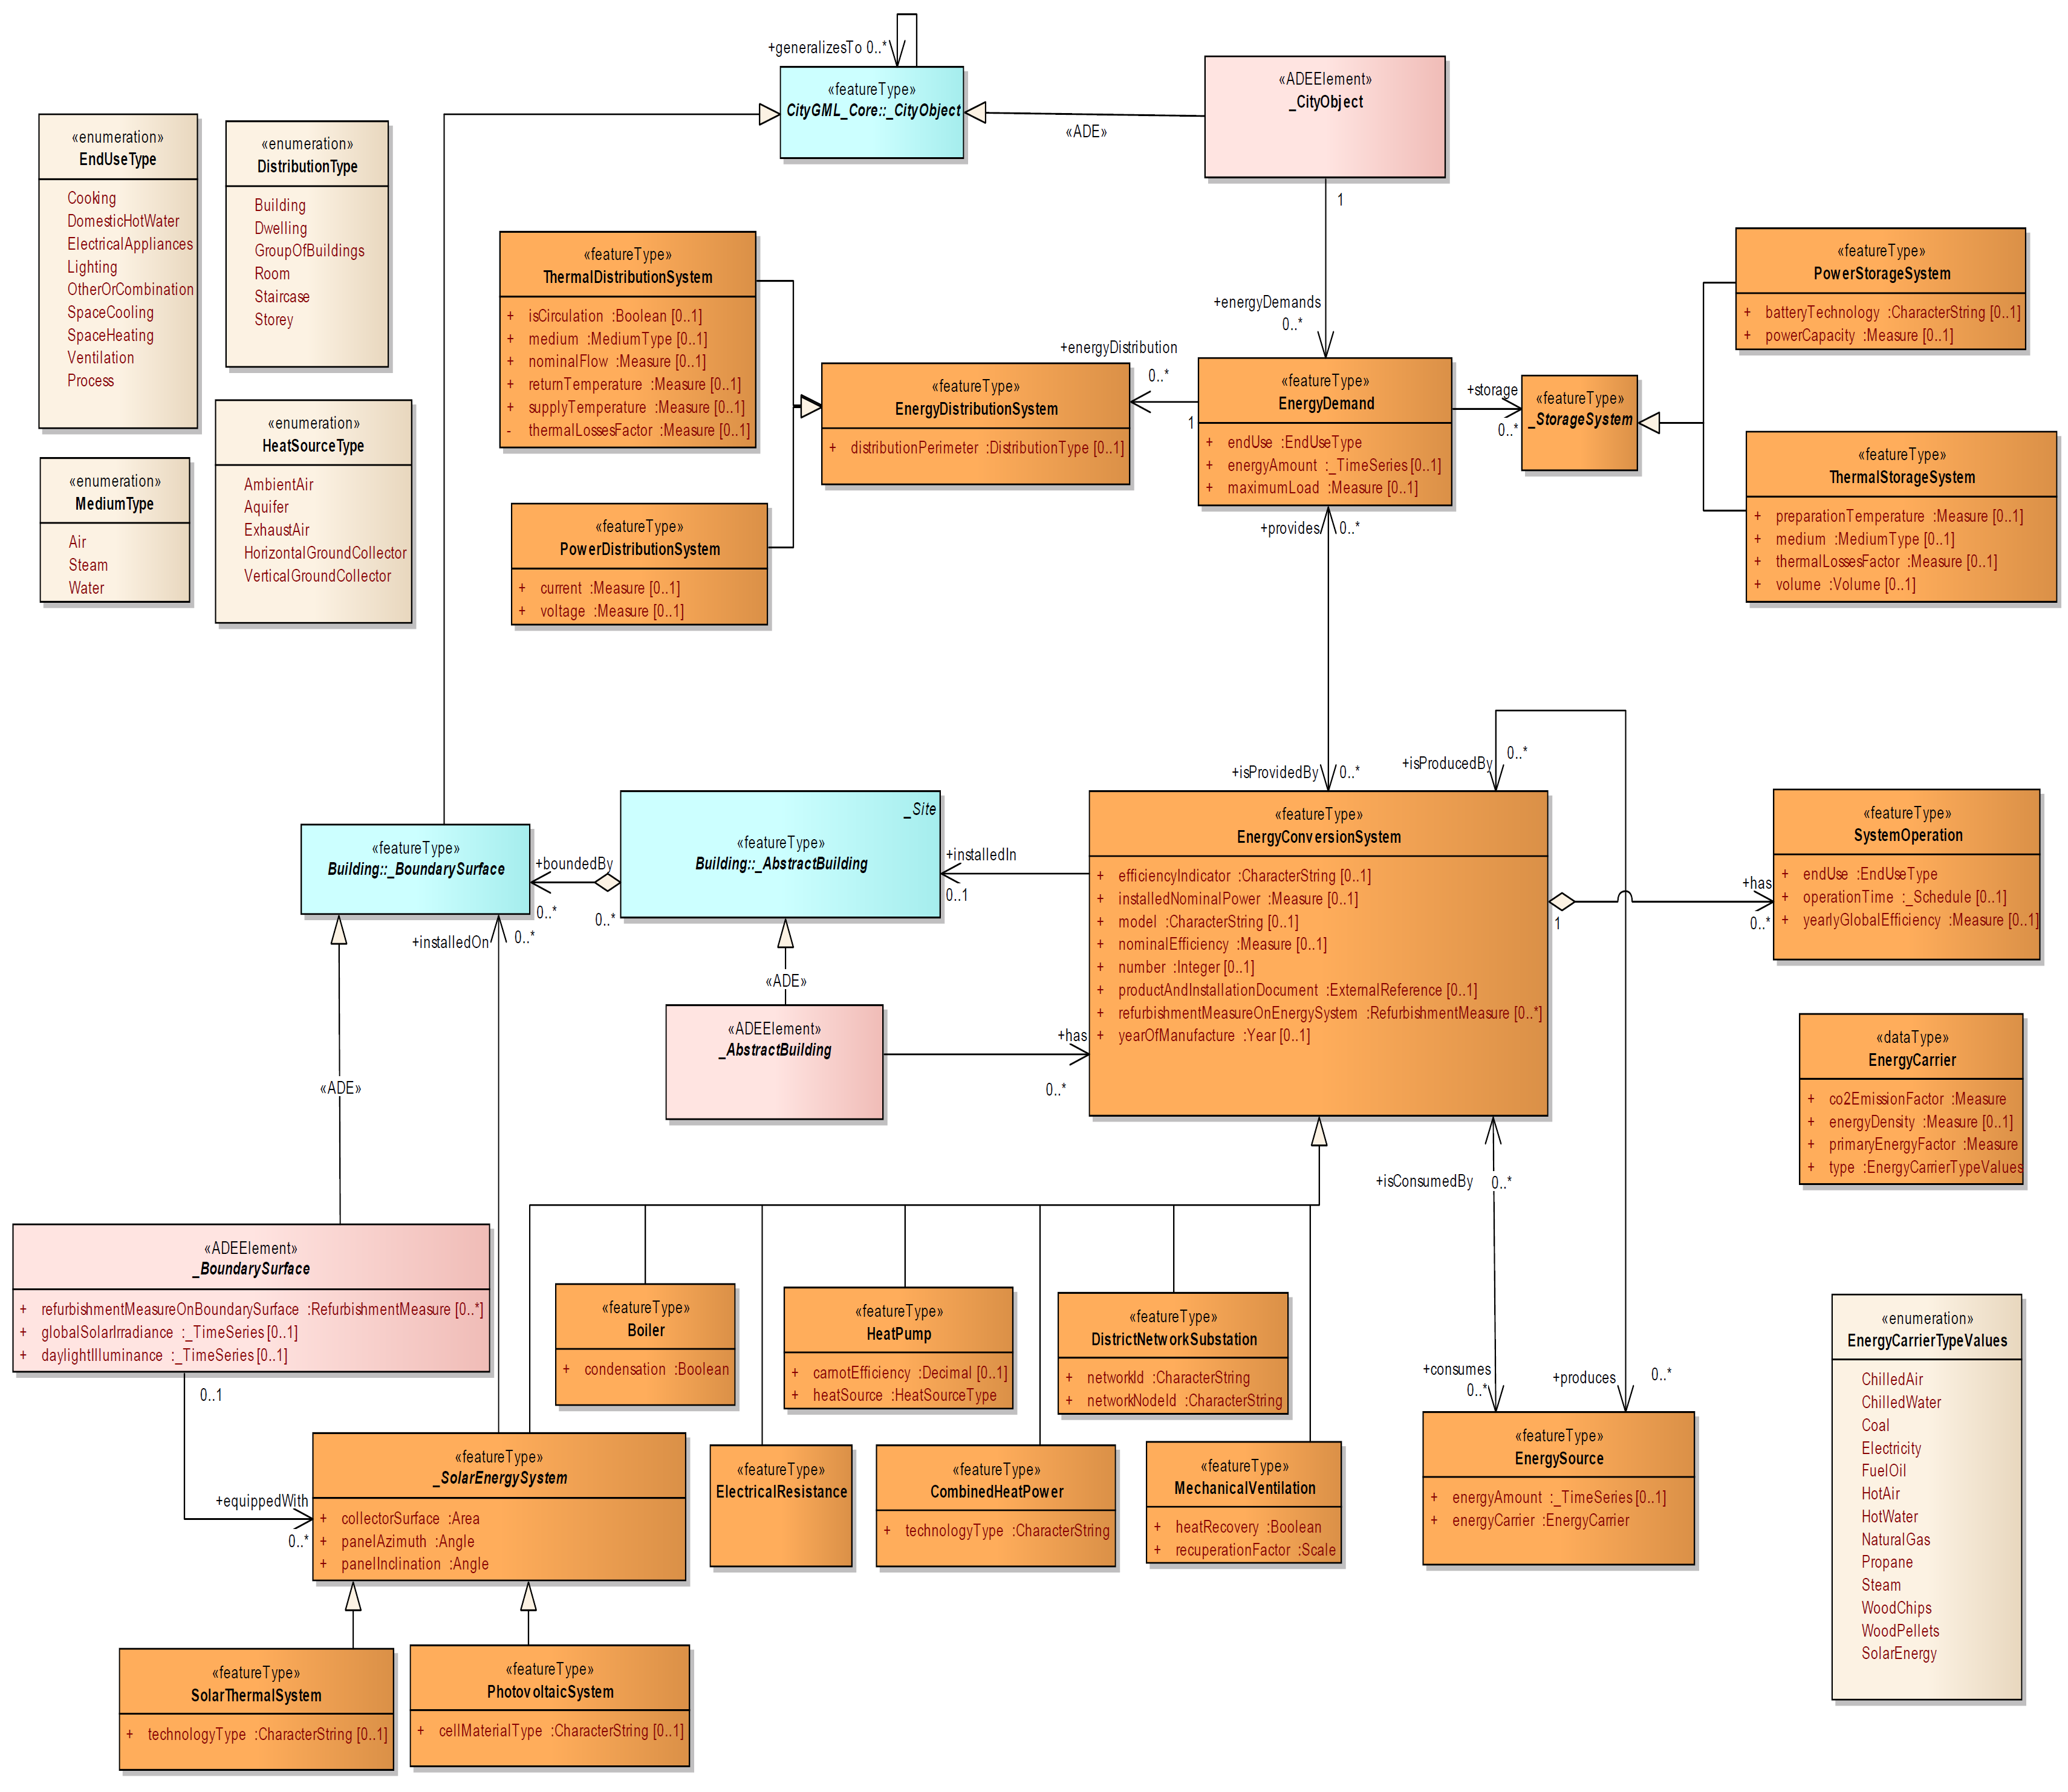
\includegraphics{fig/class_EnergySystem.png}
\caption{Class diagram of Energy System Module}
\end{figure}

The Energy System Module is a module of the ADE Energy which contains
information concerning the energy forms (energy demand, supply, sources)
and the energy systems (conversion, distribution and storage systems).
It is arranged around one central \lstinline!EnergyDemand! object.

\subsection{Energy amounts and types}\label{energy-amounts-and-types}

\subsubsection{EnergyDemand}\label{energydemand}

Useful energy required to satisfy a specific end use, such as heating,
cooling, domestic hot water etc. Beside its \lstinline!EndUseType!, this
object is characterized its \lstinline!energyAmount! (time-depending
energy demand value) and its maximum yearly load
(\lstinline!maximumLoad!) used for the sizing of the energy systems.

Every \lstinline!_CityObject! (typically
\lstinline!ADE:_AbstractBuilding!, \lstinline!ThermalZone!,
\lstinline!UsageZone! and \lstinline!BuildingUnit!) may have one or more
\lstinline!EnergyDemand!.

\subsubsection{EndUseType}\label{endusetype}

List of possible end uses as cooking, space heating and ventilation.

\subsubsection{EnergySource}\label{energysource}

Final energy consumed (and sometimes produced) by the energy conversion
system. Its energy characteristics are specified in the Energy Carrier
object.

\subsubsection{EnergyCarrier}\label{energycarrier}

Primary energy and \(CO_2\) emission factors, energy density and energy
carrier type characterize this data type for energy carriers.

\subsubsection{EnergyCarrierType}\label{energycarriertype}

List of energy carriers as coal, chilled water or electricity.

\subsection{Energy distribution}\label{energy-distribution}

\subsubsection{EnergyDistributionSystem}\label{energydistributionsystem}

System in charge of delivering the energy inside the building, from the
place of energy production to the place of end-use. Power and Thermal
distribution systems are differentiated. They all share a distribution
perimeter that is described by the distribution type.

\subsubsection{Distribution Type}\label{distribution-type}

A list of possible distribution perimeters, e.g.~Building, Dwelling,
Room.

\subsubsection{ThermalDistributionSystem}\label{thermaldistributionsystem}

Type for thermal distribution systems with attributes for circulation
(circulating system or not), the used medium, nominal flow, return and
supply temperatures and thermal losses factor.

\subsubsection{PowerDistributionSystem}\label{powerdistributionsystem}

Type for electrical distribution systems, described by current and
voltage.

\subsubsection{MediumType}\label{mediumtype}

This list is a collection of medium types as air and water.

\subsection{Energy storage}\label{energy-storage}

\subsubsection{StorageSystem}\label{storagesystem}

System storing energy. A same storage may store the energy of different
end-users and different end uses. Power and Thermal storage systems are
differentiated.

\subsubsection{ThermalStorageSystem}\label{thermalstoragesystem}

Thermal storages with a medium, preparation temperature, thermal losses
factor and a volume.

\subsubsection{PowerStorageSystem}\label{powerstoragesystem}

Electrical storages with an electrical capacity and a string to describe
the battery technology.

\subsection{Energy conversion}\label{energy-conversion}

\subsubsection{EnergyConversionSystem}\label{energyconversionsystem}

System converting an energy source into the energy necessary to satisfy
the \lstinline!EnergyDemand! (or to feed the networks).

Energy conversion systems have common parameters: efficiency indicator,
nominal installed power, nominal efficiency (in reference to an
efficiency indicator), year of manufacture, name of the model, a serial
number, a reference to product or installation documents and optionally
refurbishment measures. They may be one or more (in this case, the
nominal installed power corresponds to the totality).

Specific energy conversion systems may have in addition specific
parameters:

A same system may have several operation modes (e.g.~heat pump covering
heating and domestic hot water demands).

\subsubsection{SystemOperation}\label{systemoperation}

It details the operation of the energy conversion system for a specific
end-use and operation time. For instance, a reversible heat pump may
have 3 operation modes: heating production in winter, cooling production
in summer, and hot water production during the whole year. Attributes
are end use type, a schedule for operation time and yearly global
efficiency.

\subsubsection{DistrictNetworkSubstation}\label{districtnetworksubstation}

Subtype of \lstinline!EnergyConversionSystem! for heating or cooling
networks substations. Adds attributes for network ID and network node
ID.

\subsubsection{HeatPump}\label{heatpump}

Subtype of \lstinline!EnergyConversionSystem! for heat pumps to add
carnot efficiency and heat source. Heat source is described using a
\lstinline!HeatSourceType!.

\subsubsection{HeatSourceType}\label{heatsourcetype}

List of heat source types for heat pumps, e.g.~ambient air, aquifer and
exhaust air.

\subsubsection{ElectricalResistance}\label{electricalresistance}

Subtype of \lstinline!EnergyConversionSystem! for electrical
resistances. Comes without additional attributes.

\subsubsection{MechanicalVentilation}\label{mechanicalventilation}

Subtype of \lstinline!EnergyConversionSystem! for ventilation systems
with attributes heat recovery (with or without) and recuperation factor.

\subsubsection{CombinedHeatPower}\label{combinedheatpower}

Subtype of \lstinline!EnergyConversionSystem! for CHP systems. Utilizes
a string describing the technology type.

\subsubsection{Boiler}\label{boiler}

Subtype of \lstinline!EnergyConversionSystem! for boiler. Defines if it
is a condensation boiler or not.

\subsubsection{SolarEnergySystem}\label{solarenergysystem}

Subclass of \lstinline!EnergyConversionSystem! for solar energy systems.
Has attributes for collector surface, azimuth and inclination.
Differentiates into solar thermal and photovoltaic systems.

\subsubsection{SolarThermalSystem}\label{solarthermalsystem}

Subtype of \lstinline!SolarEnergySystem! for thermal systems. Uses a
string to describe the technology type.

\subsubsection{PhotovoltaicSystem}\label{photovoltaicsystem}

Subtype of \lstinline!SolarEnergySystem! for photovoltaic systems.
Defines the material type of photovoltaic cells with a string.

\section*{References}\label{references}
\addcontentsline{toc}{section}{References}

\hypertarget{refs}{}

\end{document}
